\chapter{Wyniki badań i ich analiza}

% TODO: poprawić po zakończeniu rozdziału
Szósty rozdział pracy przedstawia kryteria oceny wyników badań przeprowadzonych w ramach scenariuszy $\mathcal{A}$ i $\mathcal{B}$, w tym definiuje przyjęte metryki, zawiera szczegółowy opis pomiarów, prezentuje uzyskane wyniki, a także przedstawia ich analizę porównawczą i interpretację.

\section{Kryteria oceny wyników i opis użytych trybów benchmarków}
Badania zdefiniowane w ramach scenariuszy $\mathcal{A}$ i $\mathcal{B}$ przeprowadzono w postaci benchmarków. W tym celu wykorzystano narzędzie Java Microbenchmark Harness (JMH), stanowiące standardowy framework służący do przeprowadzania pomiarów wydajności aplikacji działających w środowisku JVM. Narzędzie to umożliwia wykonywanie powtarzalnych i możliwie precyzyjnych pomiarów czasu wykonania kodu, uwzględniając przy tym specyfikę działania maszyny wirtualnej Java, w~szczególności mechanizmy takie jak kompilacja Just-In-Time (JIT), optymalizacje wykonywanego kodu czy proces rozgrzewania środowiska uruchomieniowego \cite{jmh-source-code}.

\subsection{Tryb pomiaru przepustowości (\texttt{Throughput})}
Tryb \texttt{Throughput} w JMH służy do pomiaru przepustowości badanego fragmentu kodu, określając liczbę operacji wykonanych w jednostce czasu (w przypadku scenariusza $\mathcal{A}$ jednostką czasu jest sekunda). Tryb ten koncentruje się na całkowitej zdolności systemu do przetwarzania zadań przy zadanym obciążeniu, co w badanym scenariuszu pozwoliło na analizę wydajności i skalowalności różnych wariantów systemów współbieżnych. \cite{jmh-documentation}

Z powyższego opisu wynika, że metryką mierzoną przez benchmark uruchomiony w trybie \texttt{Throughput} jest \emph{przepustowość} (ozn. THRPT), czyli liczba operacji wykonanych przez badany fragment kodu w jednostce czasu. Tryb ten został użyty przy pomiarze kodu zaimplementowanego w ramach scenariusza $\mathcal{A}$.

\subsection{Tryb próbkowania czasu (\texttt{SampleTime})}
Tryb \texttt{SampleTime} w JMH służy do pomiaru czasu wykonania pojedynczych wywołań benchmarkowanej metody na podstawie próbek zbieranych w trakcie iteracji pomiarowych.
Wynikiem jest średni czas wykonania operacji wraz z oszacowaniem błędu pomiarowego. Dodatkowo JMH raportuje rozkład zebranych próbek, w tym wartości minimalne i maksymalne oraz percentyle. Wartości te pozwalają ocenić latencję i zachowanie w~ogonie rozkładu \cite{jmh-documentation}. Tryb ten został użyty przy pomiarze kodu zaimplementowanego w ramach obu scenariuszy.

Zgodnie z definicją sformułowaną przez Luszniewicza \cite{luszniewicz1970}, mianem \emph{percentyla rzędu $p$}, gdzie $p \in [0, 100]$, określa się taką wartość $x$, że co najmniej $p\%$ obserwacji ma wartość mniejszą lub równą $x$, a co najwyżej $(100-p)\%$ obserwacji ma wartość większą lub równą $x$.
Na podstawie powyższej definicji, metryką P$n$ określa się percentyl rzędu $n$ czasu wykonania badanego fragmentu kodu. Ponadto, metryką AVG określa się średni czas wykonania badanego fragmentu kodu.

\section{Szczegółowy opis pomiarów}

\subsection{Szczegóły pomiaru dla scenariusza \ensuremath{\mathcal{A}}}
\label{sec:jmh-description-scenario-A}
Każdy z trzech wariantów scenariusza $\mathcal{A}$ (\texttt{JDBC+PT}, \texttt{R2DBC}, \texttt{JDBC+VT}) został uruchomiony dla każdego z trzech zapytań (\texttt{Q1}, \texttt{Q2}, \texttt{Q3}) i na różnych poziomach współbieżności (16, 32, 64, 256, 1024) w następującej konfiguracji narzędzia JMH:
\begin{itemize}
    \itemsep0em
    \item \mintinline{java}|BenchmarkMode| -- tryby benchmarku: \texttt{Throughput} i \texttt{SampleTime},
    \item \mintinline{java}|Warmup| -- liczba iteracji rozgrzewkowych\footnote{Iteracje rozgrzewkowe pozwalają na ustabilizowanie działania środowiska uruchomieniowego JVM, m.in. poprzez aktywację kompilatora JIT i optymalizacji wykonywanego kodu, przed rozpoczęciem właściwych pomiarów. \cite{jmh-documentation}}: 5, każda trwająca 10 sekund,
    \item \mintinline{java}|Measurement| -- liczba iteracji pomiarów właściwych: 10, każda trwająca 10 sekund,
    \item \mintinline{java}|Fork| -- liczba rozgałęzień\footnote{Rozgałęzienia to liczba niezależnych uruchomień środowiska JVM, w których wykonywany jest pomiar. \cite{jmh-documentation}}: 3,
    \item \mintinline{java}|Threads| -- liczba wątków jednocześnie wykonujących kod: 1.
\end{itemize}

\newpage
\noindent
Liczba wątków w powyższej konfiguracji została ustawiona na 1 ze względu na fakt, że zarządzanie liczbą i rodzajem wątków zostało przeniesione bezpośrednio do metod, na których wykonywane są benchmarki. Parametr ten reprezentowany jest przez poziom współbieżności. Implementacja tej logiki różni się w zależności od wariantu modelu współbieżności, co zostało szczegółowo przedstawione w~sekcji \hyperref[sec:results-scenario-A]{5.2.1 Scenariusz \ensuremath{\mathcal{A}}: Integracja z bazą danych ze sterownikiem blokującym (JDBC) i reaktywnym (R2DBC)}.

W celu uniknięcia dokonania niezamierzonych optymalizacji przez środowisko JVM, każdy wariant wykorzystuje wspomniane w rozdziale piątym narzędzie \mintinline{java}|Blackhole| dostępne w ramach JMH, konsumujące wyniki obliczeń w sposób, którego kompilator nie może bezpiecznie zoptymalizować. W ten sposób narzędzie to pozwala zapewnić, że mierzony kod faktycznie zostaje wykonany, a uzyskane wyniki benchmarku odzwierciedlają rzeczywisty koszt obliczeń. \cite{jmh-blackhole}

Metrykami mierzonymi w ramach scenariusza $\mathcal{A}$ są:
\begin{itemize}
    \itemsep0em
    \item dla trybu \texttt{Throughput}: THRPT,
    \item dla trybu \texttt{SampleTime}: AVG, P50, P95 i P99.
\end{itemize}

\subsection{Szczegóły pomiaru dla scenariusza \ensuremath{\mathcal{B}}}
bla bla bla

Metrykami mierzonymi w ramach scenariusza $\mathcal{B}$ są AVG, P50, P95, P99 i P99.9.

\section{Prezentacja wyników pomiarów}

\subsection{Wyniki pomiarów w ramach scenariusza \ensuremath{\mathcal{A}}}
\label{sec:results-scenario-A}

\subsubsection{Tryb pomiaru przepustowości (\texttt{Throughput})}
Tabele \ref{table:benchmark-A-thrpt-Q1}, \ref{table:benchmark-A-thrpt-Q2} i \ref{table:benchmark-A-thrpt-Q3} oraz odpowiadające im wykresy przedstawione na rysunkach \ref{table:benchmark-A-thrpt-Q1}, \ref{table:benchmark-A-thrpt-Q2} i \ref{table:benchmark-A-thrpt-Q3} prezentują wyniki benchmarku przeprowadzonego dla scenariusza $\mathcal{A}$ w~trybie pomiaru przepustowości, tj. w trybie \texttt{Throughput}. Wartości przedstawione w~tabelach i na odpowiadających im wykresach zostały wyznaczone w zależności od wariantu modelu współbieżności, poziomu współbieżności i zapytania.

\noindent
Dodatkowe uwagi do tabel \ref{table:benchmark-A-thrpt-Q1}, \ref{table:benchmark-A-thrpt-Q2} i \ref{table:benchmark-A-thrpt-Q3}:
\begin{enumerate}[label=(\roman*)]
    \itemsep0em
    \item Wyniki we wspomnianych wyżej tabelach podane są jako liczba operacji na sekundę. Wykresy przedstawione na odpowiadających im rysunkach prezentują te dane na osi pionowej w jednostce oznaczonej jako [ops/s].
    \item Wyniki we wspomnianych wyżej tabelach przedstawione są w formacie $S \pm E$, gdzie $S$~oznacza uzyskany wynik, a~$E$ oznacza błąd pomiaru.
    \item Wyniki i wartości błędów pomiaru we wspomnianych wyżej tabelach zapisane zostały z kropką jako separatorem dziesiętnym i zmierzone z dokładnością do części tysięcznych, tj. $0.001$.
\end{enumerate}

\vspace{3cm}
\textit{Wyniki znajdują się na następnej stronie.}

\begin{figure}[p]
    \centering
    \setlength{\tabcolsep}{0.5em}
    \renewcommand{\arraystretch}{1.2}
    \begin{tabularx}{\linewidth}{|c|>{\centering\arraybackslash}X|>{\centering\arraybackslash}X|>{\centering\arraybackslash}X|}
        \hline
        \textbf{Poz. współb.} & \textbf{JDBC+PT} & \textbf{R2DBC} & \textbf{JDBC+VT} \\
        \hline
        16 & $415.881 \pm 8.497$ & $729.356 \pm 5.935$ & $733.642 \pm 13.414$ \\
        \hline
        32 & $230.098 \pm 7.511$ & $451.219 \pm 2.474$ & $489.411 \pm 2.623$ \\
        \hline
        64 & $116.672 \pm 4.463$ & $240.370 \pm 4.193$ & $250.862 \pm 0.876$ \\
        \hline
        256 & $28.871 \pm 1.067$ & $67.178 \pm 0.352$ & $66.336 \pm 0.378$ \\
        \hline
        1024 & $6.694 \pm 0.306$ & $17.139 \pm 0.105$ & $16.782 \pm 0.111$ \\
        \hline
    \end{tabularx}
    \captionof{table}{Wartości przepustowości dla zapytania \texttt{Q1} w~ramach scenariusza $\mathcal{A}$ w~zależności od poziomu współbieżności i wariantu modelu współbieżności}
    \source{opracowanie własne}
    \label{table:benchmark-A-thrpt-Q1}
    \vspace{0.5cm} % Odstęp między tabelą a wykresami

    % --- WYKRESY ---
    \begin{subfigure}[b]{0.49\textwidth}
        \centering
        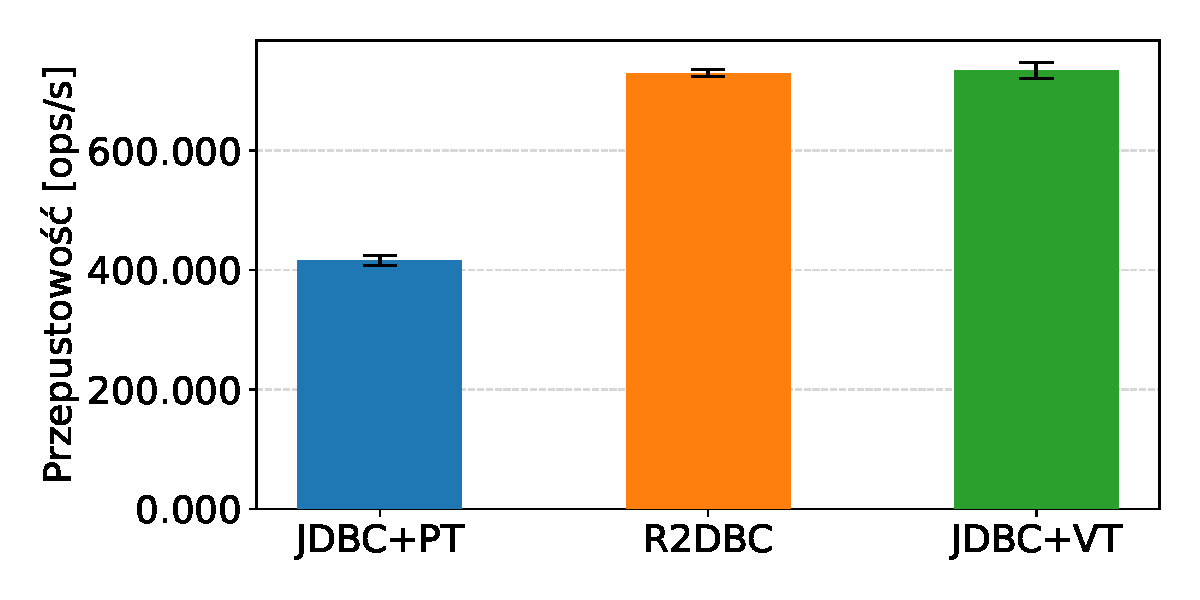
\includegraphics[width=\textwidth]{rozdzialy/rozdzial6/wykresy/A_plot_thrpt_Q1_16.pdf}
        \caption{poziom współbieżności: 16}
    \end{subfigure}
    \hfill
    \begin{subfigure}[b]{0.49\textwidth}
        \centering
        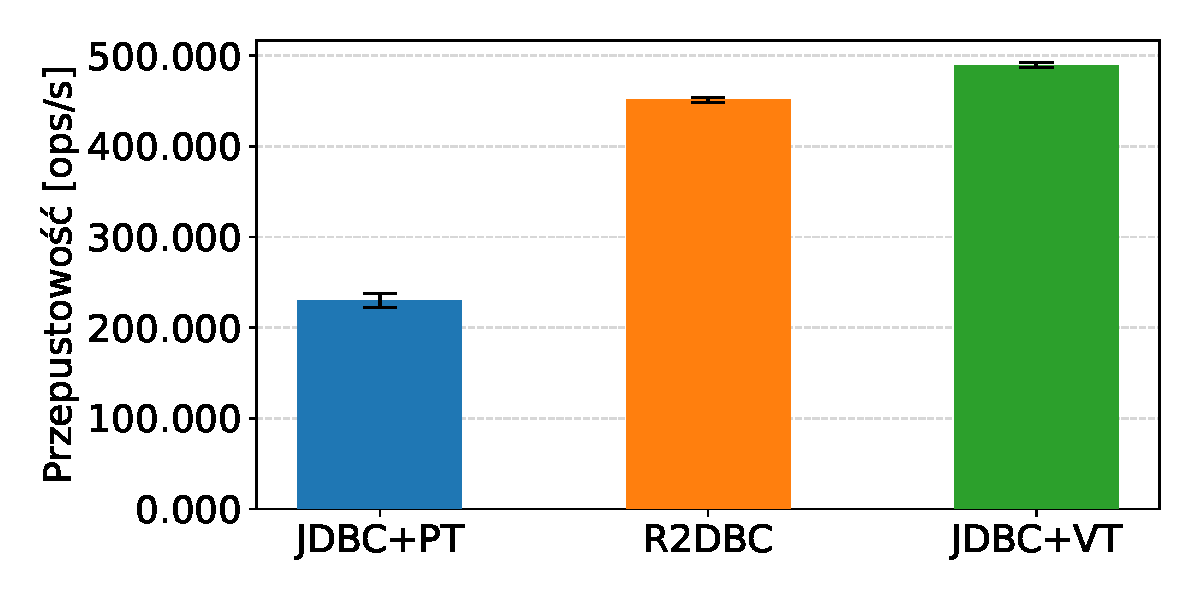
\includegraphics[width=\textwidth]{rozdzialy/rozdzial6/wykresy/A_plot_thrpt_Q1_32.pdf}
        \caption{poziom współbieżności: 32}
    \end{subfigure}

    \vspace{0.2cm}

    \begin{subfigure}[b]{0.49\textwidth}
        \centering
        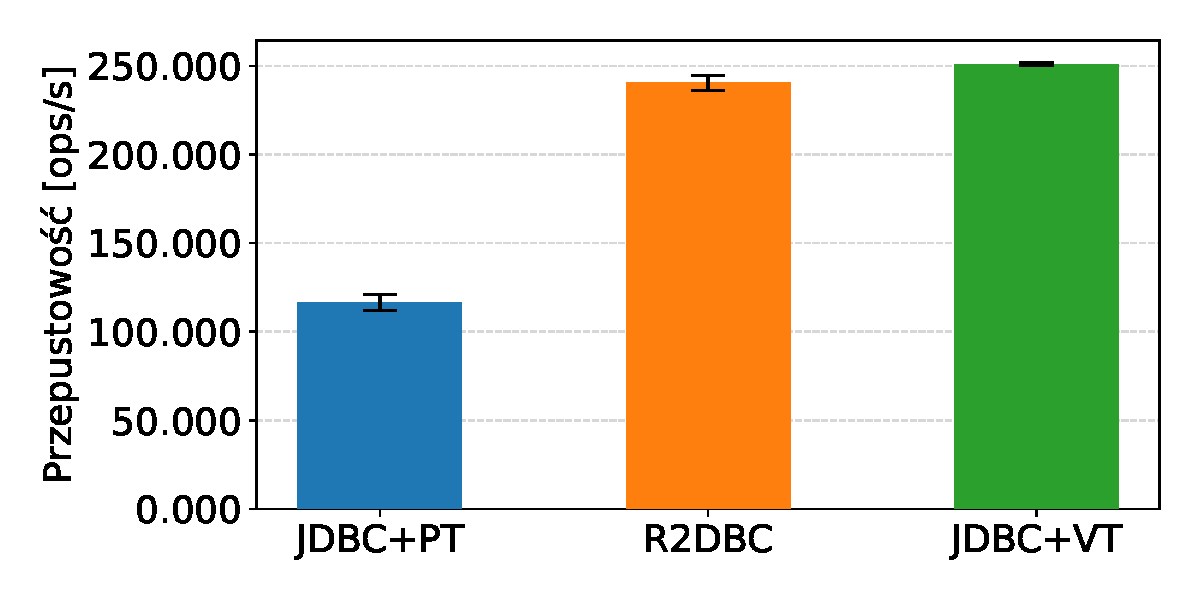
\includegraphics[width=\textwidth]{rozdzialy/rozdzial6/wykresy/A_plot_thrpt_Q1_64.pdf}
        \caption{poziom współbieżności: 64}
    \end{subfigure}
    \hfill
    \begin{subfigure}[b]{0.49\textwidth}
        \centering
        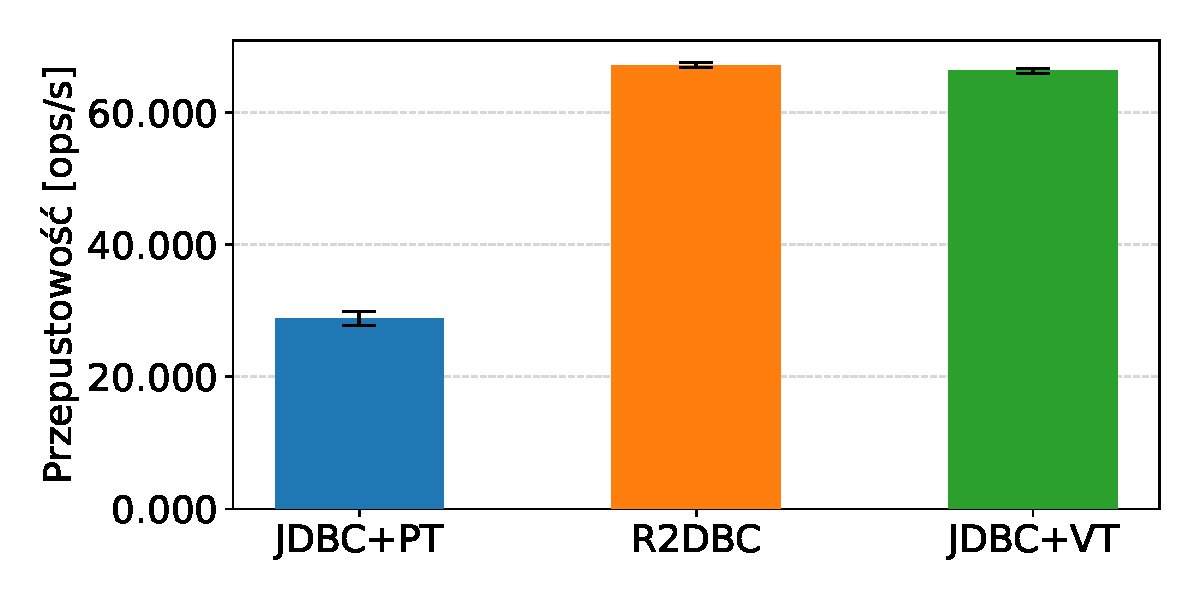
\includegraphics[width=\textwidth]{rozdzialy/rozdzial6/wykresy/A_plot_thrpt_Q1_256.pdf}
        \caption{poziom współbieżności: 256}
    \end{subfigure}

    \vspace{0.2cm}

    \begin{subfigure}[b]{0.49\textwidth}
        \centering
        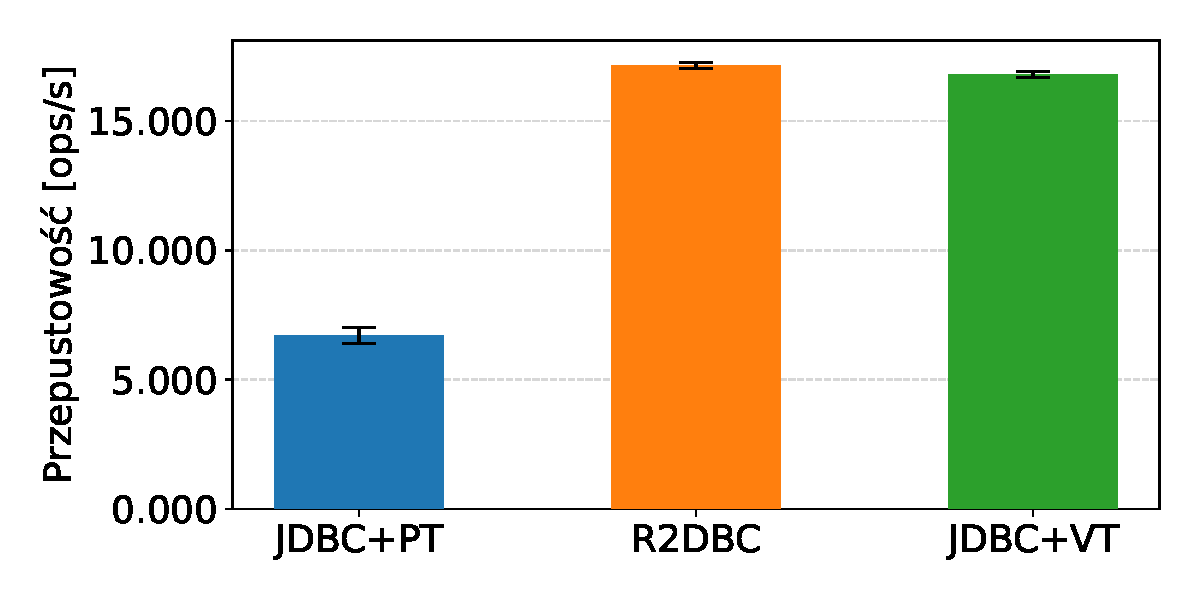
\includegraphics[width=\textwidth]{rozdzialy/rozdzial6/wykresy/A_plot_thrpt_Q1_1024.pdf}
        \caption{poziom współbieżności: 1024}
    \end{subfigure}

    \captionof{figure}{Wykresy kolumnowe przepustowości dla zapytania \texttt{Q1} w ramach scenariusza $\mathcal{A}$ w zależności od poziomu współbieżności i wariantu modelu współbieżności}
    \source{opracowanie własne}
    \label{fig:benchmark-A-thrpt-Q1}
\end{figure}

\begin{figure}[p]
    \centering
    \setlength{\tabcolsep}{0.5em}
    \renewcommand{\arraystretch}{1.2}
    \begin{tabularx}{\linewidth}{|c|>{\centering\arraybackslash}X|>{\centering\arraybackslash}X|>{\centering\arraybackslash}X|}
        \hline
        \textbf{Poz. współb.} & \textbf{JDBC+PT} & \textbf{R2DBC} & \textbf{JDBC+VT} \\
        \hline
        16 & $142.817 \pm 24.898$ & $174.474 \pm 36.850$ & $159.069 \pm 33.964$ \\
        \hline
        32 & $107.766 \pm 14.097$ & $122.683 \pm 0.635$ & $157.456 \pm 29.941$ \\
        \hline
        64 & $55.572 \pm 5.507$ & $74.120 \pm 10.150$ & $70.235 \pm 4.447$ \\
        \hline
        256 & $14.765 \pm 1.268$ & $19.392 \pm 2.232$ & $19.884 \pm 1.825$ \\
        \hline
        1024 & $3.736 \pm 0.365$ & $4.600 \pm 0.031$ & $5.042 \pm 0.379$ \\
        \hline
    \end{tabularx}
    \captionof{table}{Wartości przepustowości dla zapytania \texttt{Q2} w ramach scenariusza $\mathcal{A}$ w~zależności od poziomu współbieżności i wariantu modelu współbieżności}
    \source{opracowanie własne}
    \label{table:benchmark-A-thrpt-Q2}
    \vspace{0.5cm} % Odstęp między tabelą a wykresami

    % --- WYKRESY ---
    \begin{subfigure}[b]{0.49\textwidth}
        \centering
        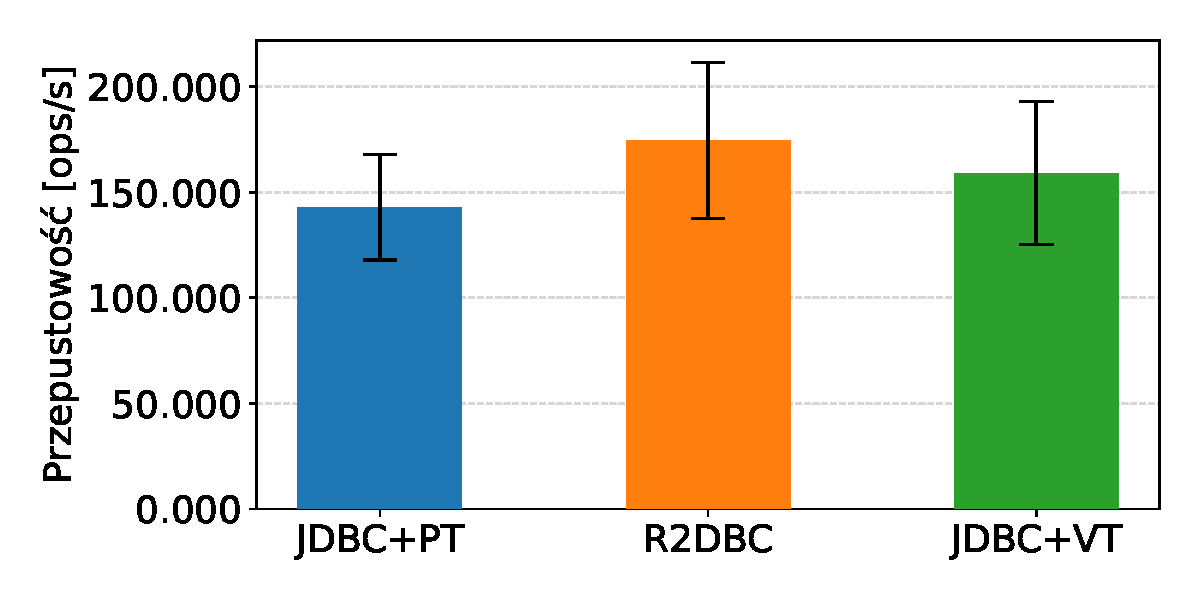
\includegraphics[width=\textwidth]{rozdzialy/rozdzial6/wykresy/A_plot_thrpt_Q2_16.pdf}
        \caption{poziom współbieżności: 16}
    \end{subfigure}
    \hfill
    \begin{subfigure}[b]{0.49\textwidth}
        \centering
        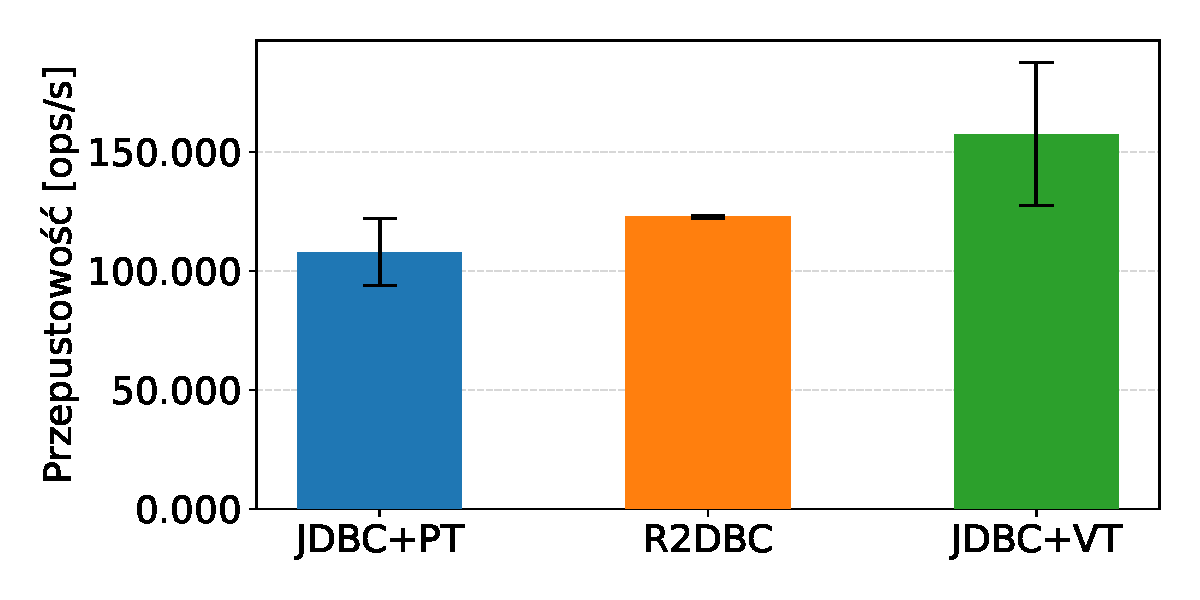
\includegraphics[width=\textwidth]{rozdzialy/rozdzial6/wykresy/A_plot_thrpt_Q2_32.pdf}
        \caption{poziom współbieżności: 32}
    \end{subfigure}

    \vspace{0.2cm}

    \begin{subfigure}[b]{0.49\textwidth}
        \centering
        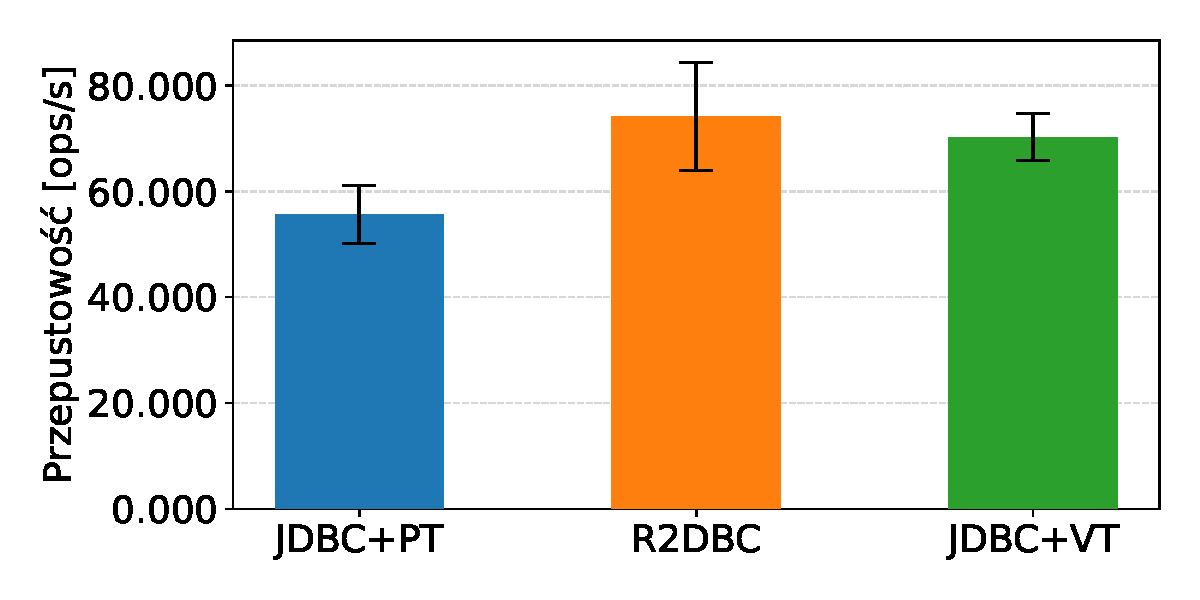
\includegraphics[width=\textwidth]{rozdzialy/rozdzial6/wykresy/A_plot_thrpt_Q2_64.pdf}
        \caption{poziom współbieżności: 64}
    \end{subfigure}
    \hfill
    \begin{subfigure}[b]{0.49\textwidth}
        \centering
        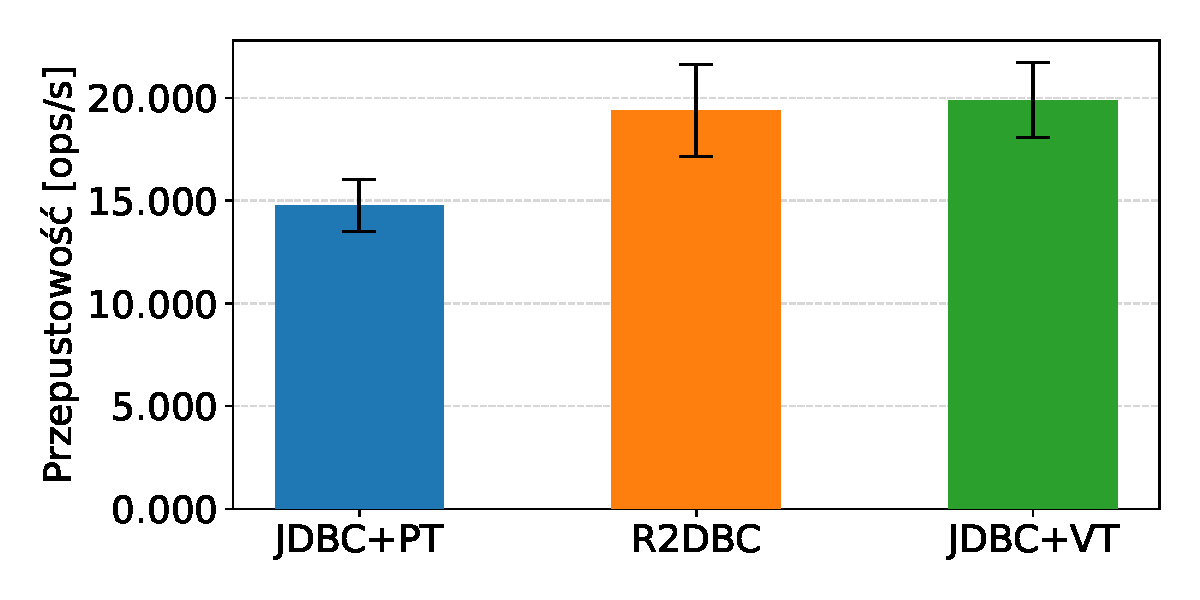
\includegraphics[width=\textwidth]{rozdzialy/rozdzial6/wykresy/A_plot_thrpt_Q2_256.pdf}
        \caption{poziom współbieżności: 256}
    \end{subfigure}

    \vspace{0.2cm}

    \begin{subfigure}[b]{0.49\textwidth}
        \centering
        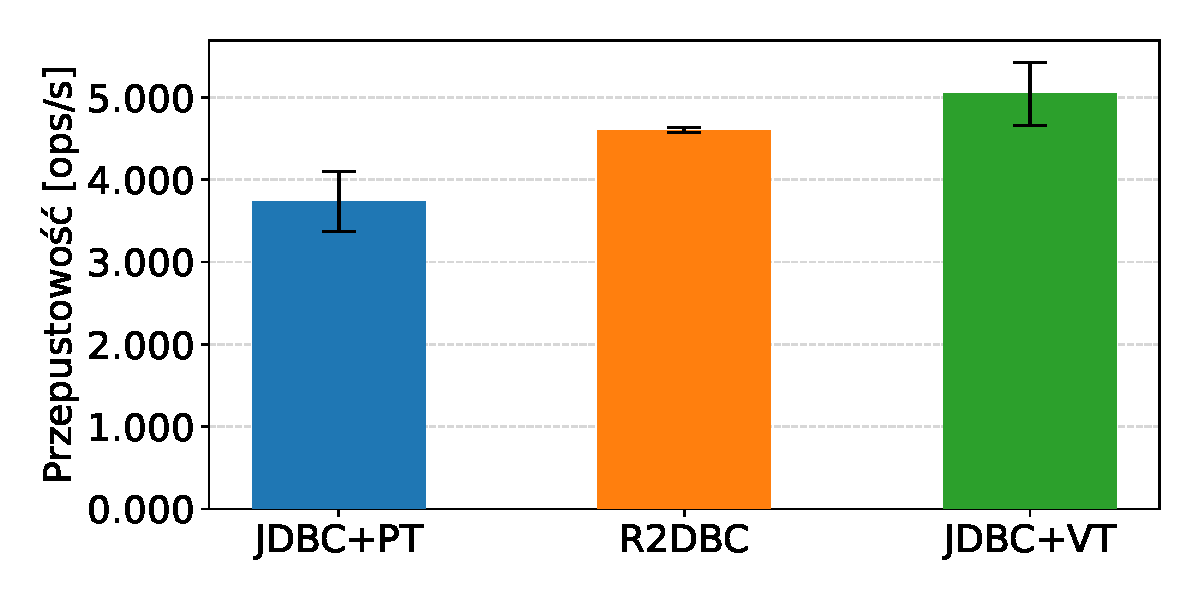
\includegraphics[width=\textwidth]{rozdzialy/rozdzial6/wykresy/A_plot_thrpt_Q2_1024.pdf}
        \caption{poziom współbieżności: 1024}
    \end{subfigure}

    \captionof{figure}{Wykresy kolumnowe przepustowości dla zapytania \texttt{Q2} w ramach scenariusza $\mathcal{A}$ w zależności od poziomu współbieżności i wariantu modelu współbieżności}
    \source{opracowanie własne}
    \label{fig:benchmark-A-thrpt-Q2}
\end{figure}

\begin{figure}[p]
    \centering
    \setlength{\tabcolsep}{0.5em}
    \renewcommand{\arraystretch}{1.2}
    \begin{tabularx}{\linewidth}{|c|>{\centering\arraybackslash}X|>{\centering\arraybackslash}X|>{\centering\arraybackslash}X|}
        \hline
        \textbf{Poz. współb.} & \textbf{JDBC+PT} & \textbf{R2DBC} & \textbf{JDBC+VT} \\
        \hline
        16 & $4.943 \pm 0.020$ & $5.003 \pm 0.027$ & $4.940 \pm 0.027$ \\
        \hline
        32 & $2.667 \pm 0.009$ & $2.705 \pm 0.011$ & $2.673 \pm 0.010$ \\
        \hline
        64 & $1.319 \pm 0.004$ & $1.332 \pm 0.006$ & $1.314 \pm 0.008$ \\
        \hline
        256 & $0.330 \pm 0.002$ & $0.335 \pm 0.001$ & $0.330 \pm 0.002$ \\
        \hline
        1024 & $0.187 \pm 0.001$ & $0.084 \pm 0.001$ & $0.192 \pm 0.001$ \\
        \hline
    \end{tabularx}
    \captionof{table}{Wartości przepustowości dla zapytania \texttt{Q3} w ramach scenariusza $\mathcal{A}$ w~zależności od poziomu współbieżności i wariantu modelu współbieżności}
    \source{opracowanie własne}
    \label{table:benchmark-A-thrpt-Q3}

    \vspace{0.5cm} % Odstęp między tabelą a wykresami

    % --- WYKRESY ---
    \begin{subfigure}[b]{0.49\textwidth}
        \centering
        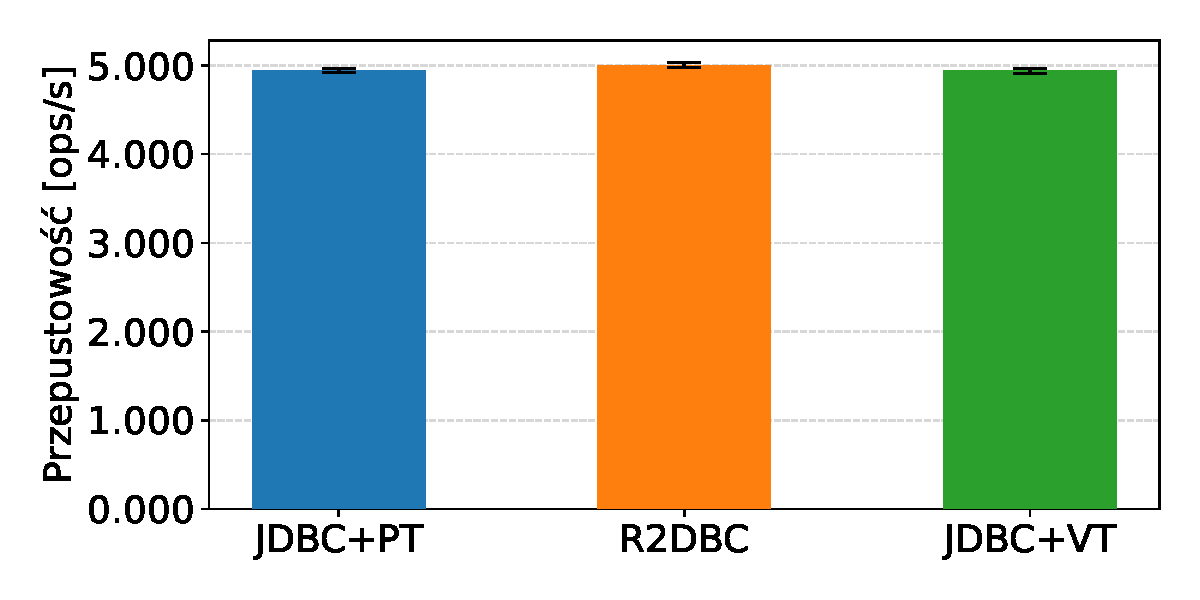
\includegraphics[width=\textwidth]{rozdzialy/rozdzial6/wykresy/A_plot_thrpt_Q3_16.pdf}
        \caption{poziom współbieżności: 16}
    \end{subfigure}
    \hfill
    \begin{subfigure}[b]{0.49\textwidth}
        \centering
        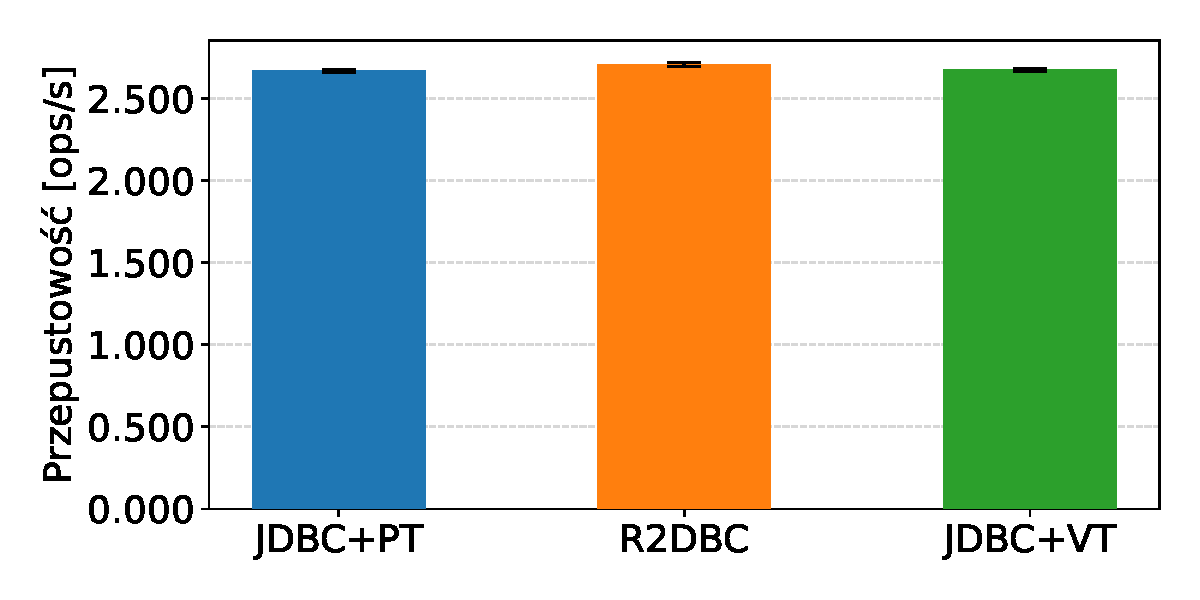
\includegraphics[width=\textwidth]{rozdzialy/rozdzial6/wykresy/A_plot_thrpt_Q3_32.pdf}
        \caption{poziom współbieżności: 32}
    \end{subfigure}

    \vspace{0.2cm}

    \begin{subfigure}[b]{0.49\textwidth}
        \centering
        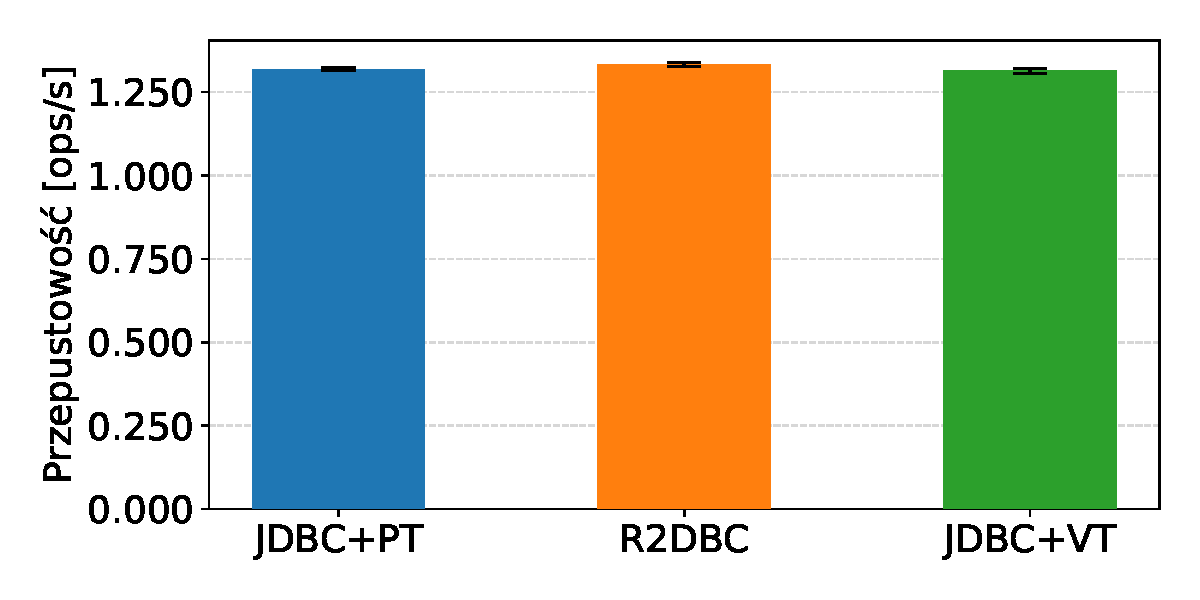
\includegraphics[width=\textwidth]{rozdzialy/rozdzial6/wykresy/A_plot_thrpt_Q3_64.pdf}
        \caption{poziom współbieżności: 64}
    \end{subfigure}
    \hfill
    \begin{subfigure}[b]{0.49\textwidth}
        \centering
        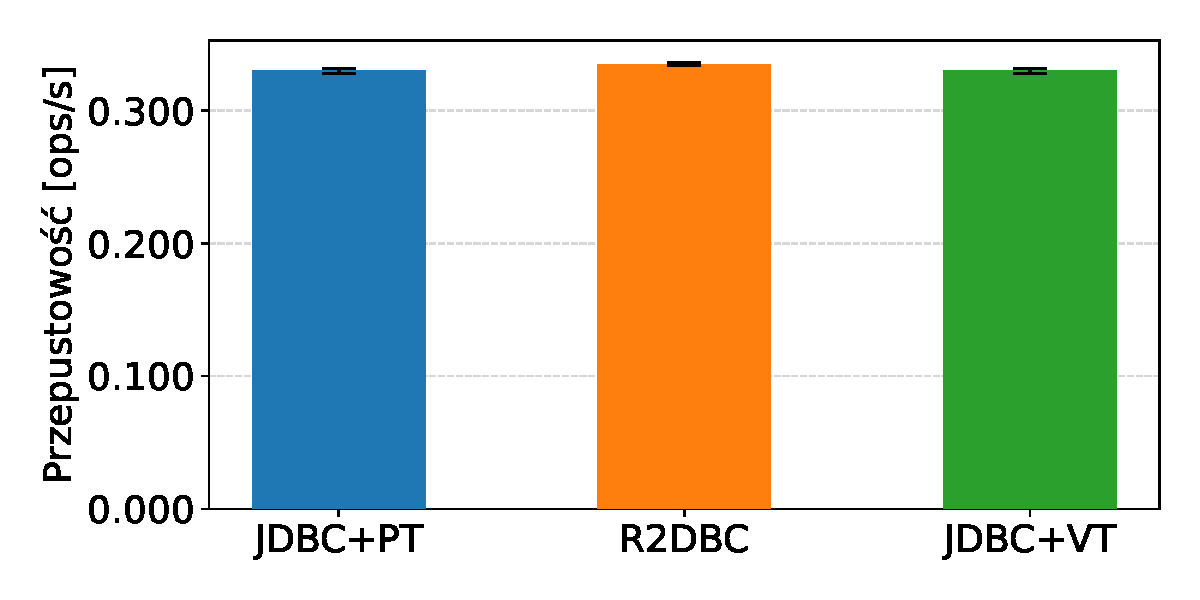
\includegraphics[width=\textwidth]{rozdzialy/rozdzial6/wykresy/A_plot_thrpt_Q3_256.pdf}
        \caption{poziom współbieżności: 256}
    \end{subfigure}

    \vspace{0.2cm}

    \begin{subfigure}[b]{0.49\textwidth}
        \centering
        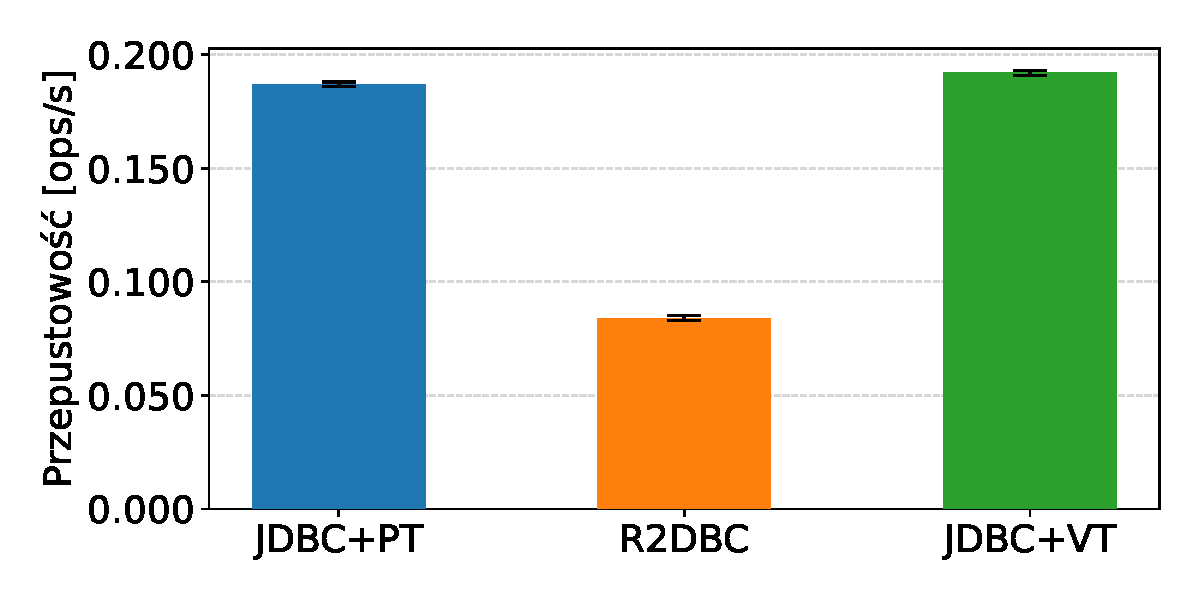
\includegraphics[width=\textwidth]{rozdzialy/rozdzial6/wykresy/A_plot_thrpt_Q3_1024.pdf}
        \caption{poziom współbieżności: 1024}
    \end{subfigure}

    \captionof{figure}{Wykresy kolumnowe przepustowości dla zapytania \texttt{Q3} w ramach scenariusza $\mathcal{A}$ w zależności od poziomu współbieżności i wariantu modelu współbieżności}
    \source{opracowanie własne}
    \label{fig:benchmark-A-thrpt-Q3}
\end{figure}

\newpage
\subsubsection{Tryb próbkowania czasu (\texttt{SampleTime})}

Dodatkowe uwagi do tabel \ref{table:benchmark-A-sample-Q1}, \ref{table:benchmark-A-sample-Q2} i \ref{table:benchmark-A-sample-Q3}:
\begin{enumerate}[label=(\roman*)]
    \item Wyniki we wspomnianych wyżej tabelach uwzględniają średni czas (AVG) i wartości percentyli P50, P95, P99 czasu wykonania badanych wariantów scenariusza i podane są w sekundach. Wykresy przedstawione na na odpowiadających im rysunkach prezentują te dane na osi pionowej w jednostce oznaczonej jako [s].
    \item Wyniki we wierszach oznaczonych przez AVG we wspomnianych wyżej tabelach są przedstawione w formacie $S \pm E$, gdzie $S$ oznacza uzyskany wynik, a~$E$ oznacza błąd pomiaru.
    \item Wyniki i wartości błędów we wspomnianych wyżej tabelach zapisane zostały z kropką jako separatorem dziesiętnym, z dokładnością do części tysięcznych, tj. $0.001$.
\end{enumerate}

\vspace{3cm}
\textit{Wyniki znajdują się na następnej stronie.}

\setlength{\tabcolsep}{0.5em} % for the horizontal padding
\renewcommand{\arraystretch}{1.2} % for the vertical padding
\begin{table}[p]
    \centering
    \setlength{\tabcolsep}{0.5em}
    \renewcommand{\arraystretch}{1.2}
    \begin{tabularx}{\linewidth}{|c|c|>{\centering\arraybackslash}X|>{\centering\arraybackslash}X|>{\centering\arraybackslash}X|}
        \hline
        \textbf{Poz. współb.} & \textbf{Metryka} & \textbf{JDBC + PT} & \textbf{R2DBC} & \textbf{JDBC + VT} \\
        \hline
        \multirow{4}{*}{16} & AVG & $0.003 \pm 0.001$ & $0.001 \pm 0.001$ & $0.001 \pm 0.001$ \\ \cline{2-5}
                            & P50 & 0.003 & 0.001 & 0.001 \\ \cline{2-5}
                            & P95 & 0.003 & 0.002 & 0.002 \\ \cline{2-5}
                            & P99 & 0.004 & 0.002 & 0.002 \\
        \hline
        \multirow{4}{*}{32} & AVG & $0.004 \pm 0.001$ & $0.002 \pm 0.001$ & $0.002 \pm 0.001$ \\ \cline{2-5}
                            & P50 & 0.004 & 0.002 & 0.002 \\ \cline{2-5}
                            & P95 & 0.005 & 0.003 & 0.002 \\ \cline{2-5}
                            & P99 & 0.006 & 0.004 & 0.003 \\
        \hline
        \multirow{4}{*}{64} & AVG & $0.009 \pm 0.001$ & $0.004 \pm 0.001$ & $0.004 \pm 0.001$ \\ \cline{2-5}
                            & P50 & 0.009 & 0.004 & 0.004 \\ \cline{2-5}
                            & P95 & 0.010 & 0.005 & 0.005 \\ \cline{2-5}
                            & P99 & 0.011 & 0.006 & 0.006 \\
        \hline
        \multirow{4}{*}{256} & AVG & $0.036 \pm 0.001$ & $0.015 \pm 0.001$ & $0.015 \pm 0.001$ \\ \cline{2-5}
                             & P50 & 0.035 & 0.015 & 0.015 \\ \cline{2-5}
                             & P95 & 0.039 & 0.017 & 0.018 \\ \cline{2-5}
                             & P99 & 0.043 & 0.020 & 0.020 \\
        \hline
        \multirow{4}{*}{1024} & AVG & $0.159 \pm 0.001$ & $0.058 \pm 0.001$ & $0.060 \pm 0.001$ \\ \cline{2-5}
                              & P50 & 0.158 & 0.057 & 0.058 \\ \cline{2-5}
                              & P95 & 0.177 & 0.065 & 0.066 \\ \cline{2-5}
                              & P99 & 0.187 & 0.070 & 0.071 \\
        \hline
    \end{tabularx}
    \caption{Wartości średniego czasu i percentyli P50, P95, P99 dla zapytania \texttt{Q1} w~ramach scenariusza $\mathcal{A}$ w~zależności od poziomu współbieżności i~wariantu modelu współbieżności}
    \source{opracowanie własne}
    \label{table:benchmark-A-sample-Q1}
\end{table}

    % \begin{subfigure}[b]{0.49\textwidth}
    %     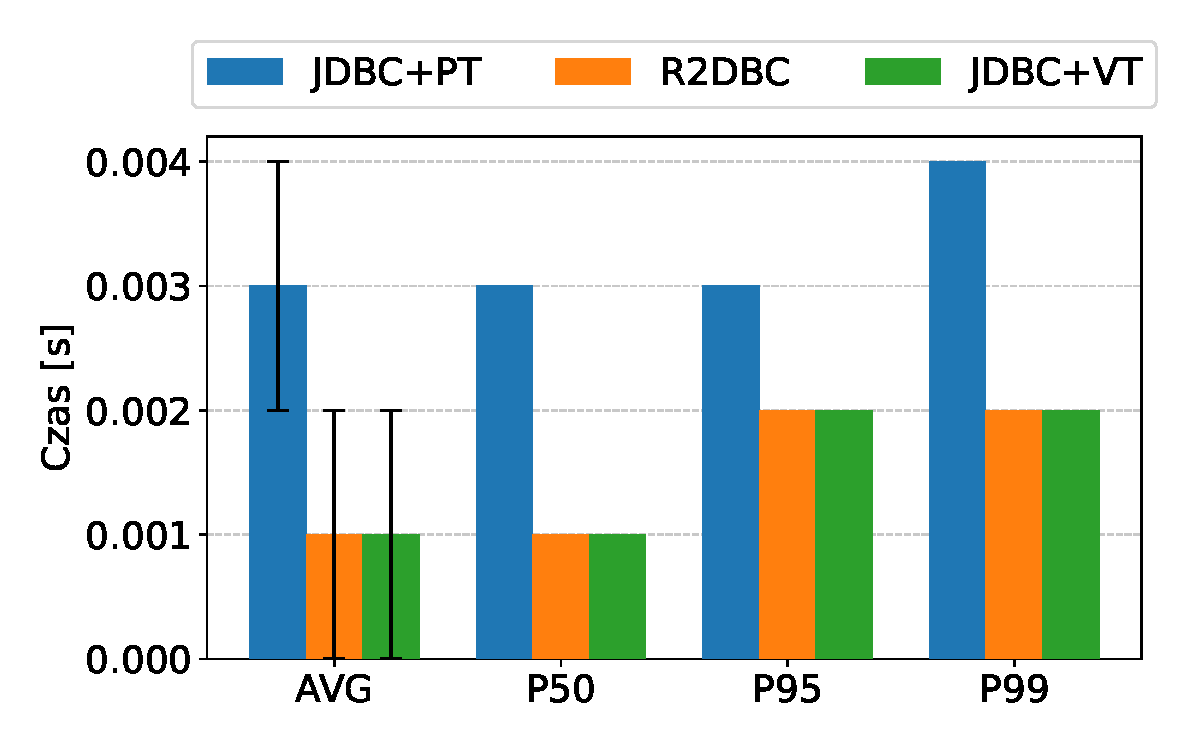
\includegraphics[width=\textwidth]{rozdzialy/rozdzial6/wykresy/A_plot_avg_Q1_16.pdf}
    %     \caption{poziom współbieżności: 16}
    %     \label{fig:benchmark-A-sample-Q1-16}
    % \end{subfigure}
    % \hfill
    % \begin{subfigure}[b]{0.49\textwidth}
    %     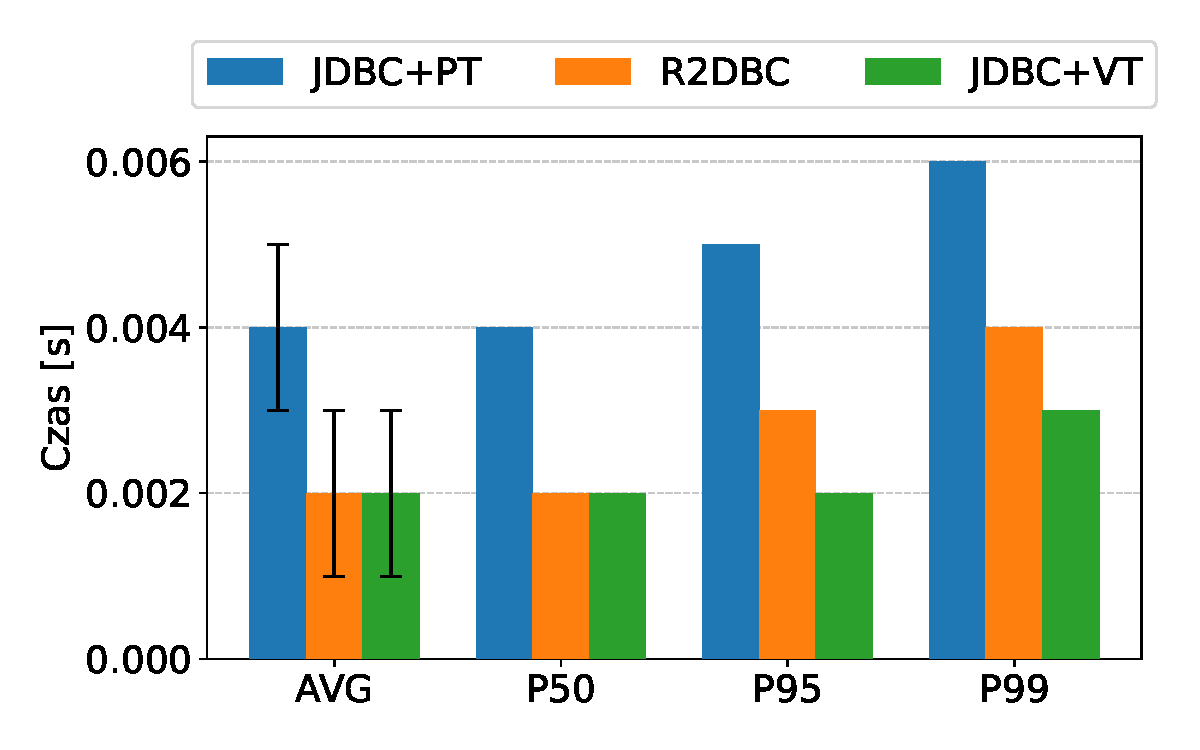
\includegraphics[width=\textwidth]{rozdzialy/rozdzial6/wykresy/A_plot_avg_Q1_32.pdf}
    %     \caption{poziom współbieżności: 32}
    %     \label{fig:benchmark-A-sample-Q1-32}
    % \end{subfigure}

    % \vspace{0.5cm}

    % \begin{subfigure}[b]{0.49\textwidth}
    %     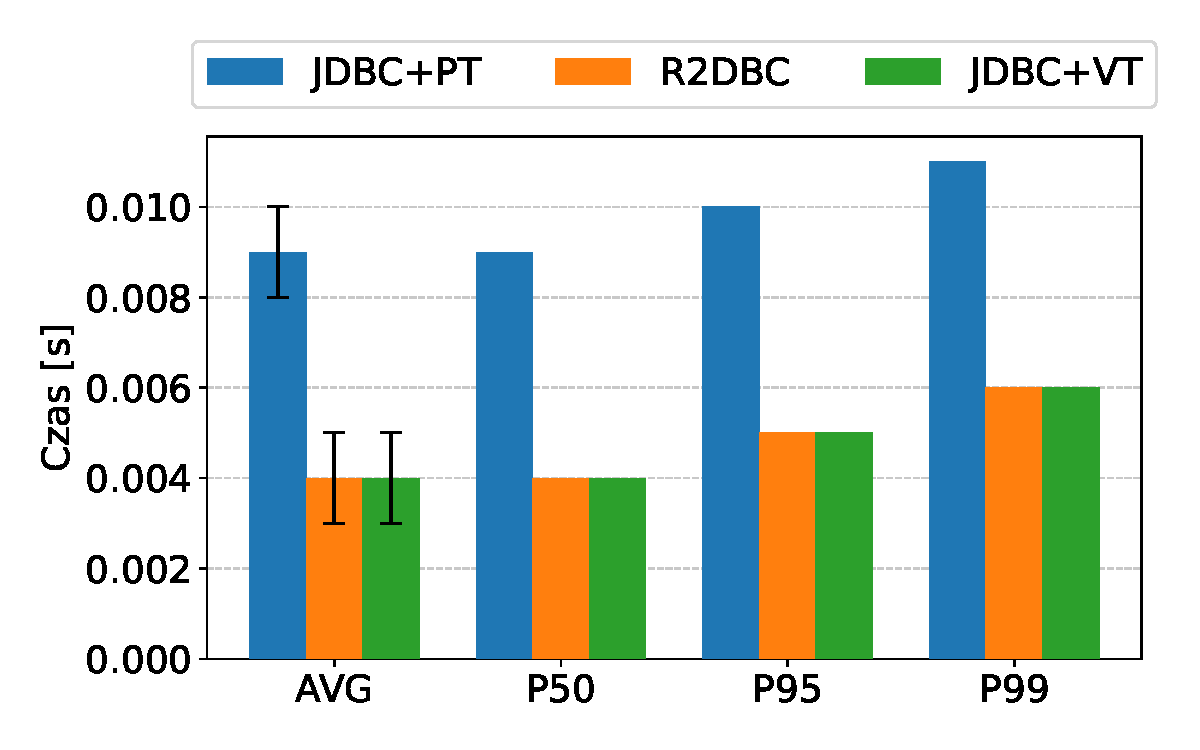
\includegraphics[width=\textwidth]{rozdzialy/rozdzial6/wykresy/A_plot_avg_Q1_64.pdf}
    %     \caption{poziom współbieżności: 64}
    %     \label{fig:benchmark-A-sample-Q1-64}
    % \end{subfigure}
    % \hfill
    % \begin{subfigure}[b]{0.49\textwidth}
    %     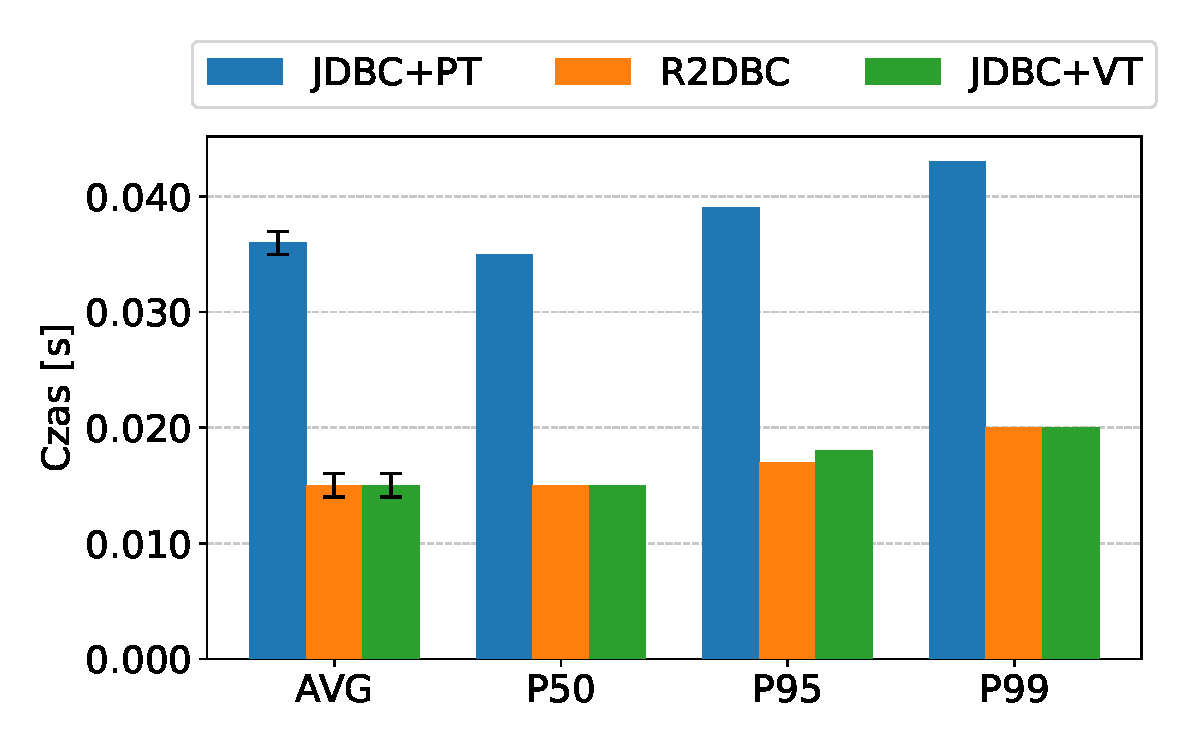
\includegraphics[width=\textwidth]{rozdzialy/rozdzial6/wykresy/A_plot_avg_Q1_256.pdf}
    %     \caption{poziom współbieżności: 256}
    %     \label{fig:benchmark-A-sample-Q1-256}
    % \end{subfigure}

    % \vspace{0.5cm}

    % \begin{subfigure}[b]{0.49\textwidth}
    %     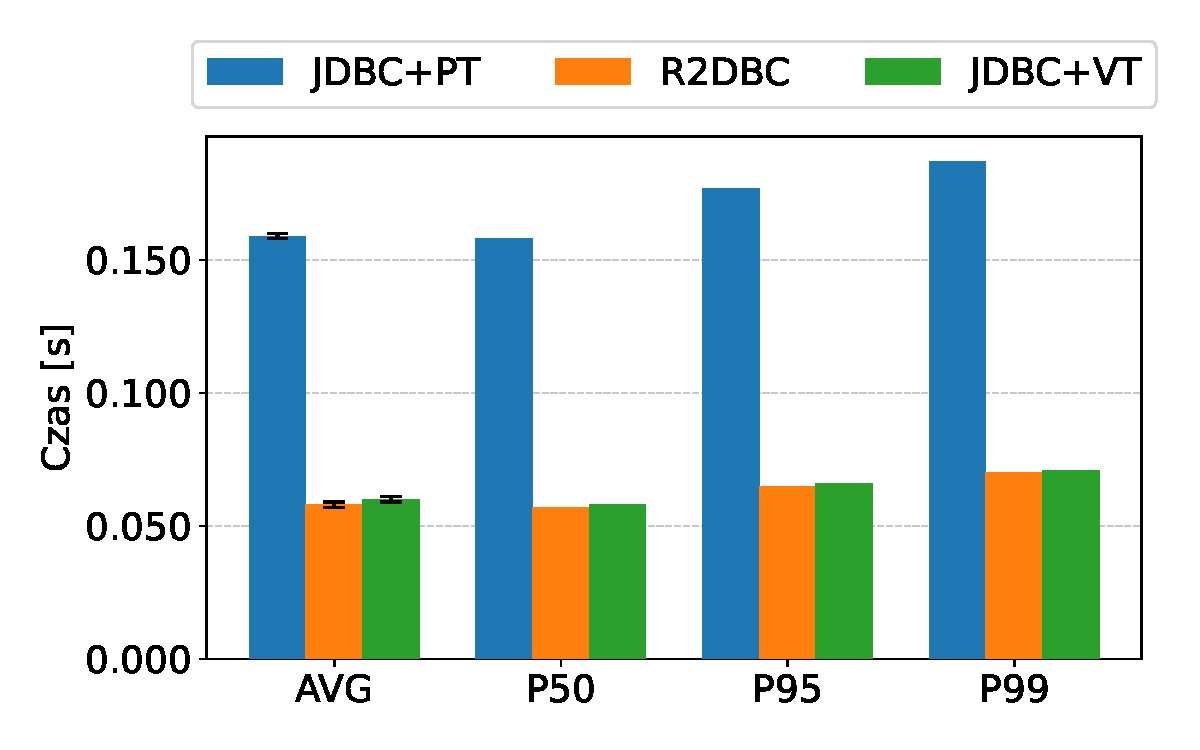
\includegraphics[width=\textwidth]{rozdzialy/rozdzial6/wykresy/A_plot_avg_Q1_1024.pdf}
    %     \caption{poziom współbieżności: 1024}
    %     \label{fig:benchmark-A-sample-Q1-1024}
    % \end{subfigure}
    % \captionof{figure}{Wykresy kolumnowe średniego czasu i latencji P50, P95, P99 dla różnych modeli współbieżności w scenariuszu A dla zapytania \texttt{Q1}}
    % \source{opracowanie własne}
    % \label{fig:benchmark-A-sample-Q1}

\begin{figure}[p]
    \centering
    \begin{subfigure}[b]{0.49\textwidth}
        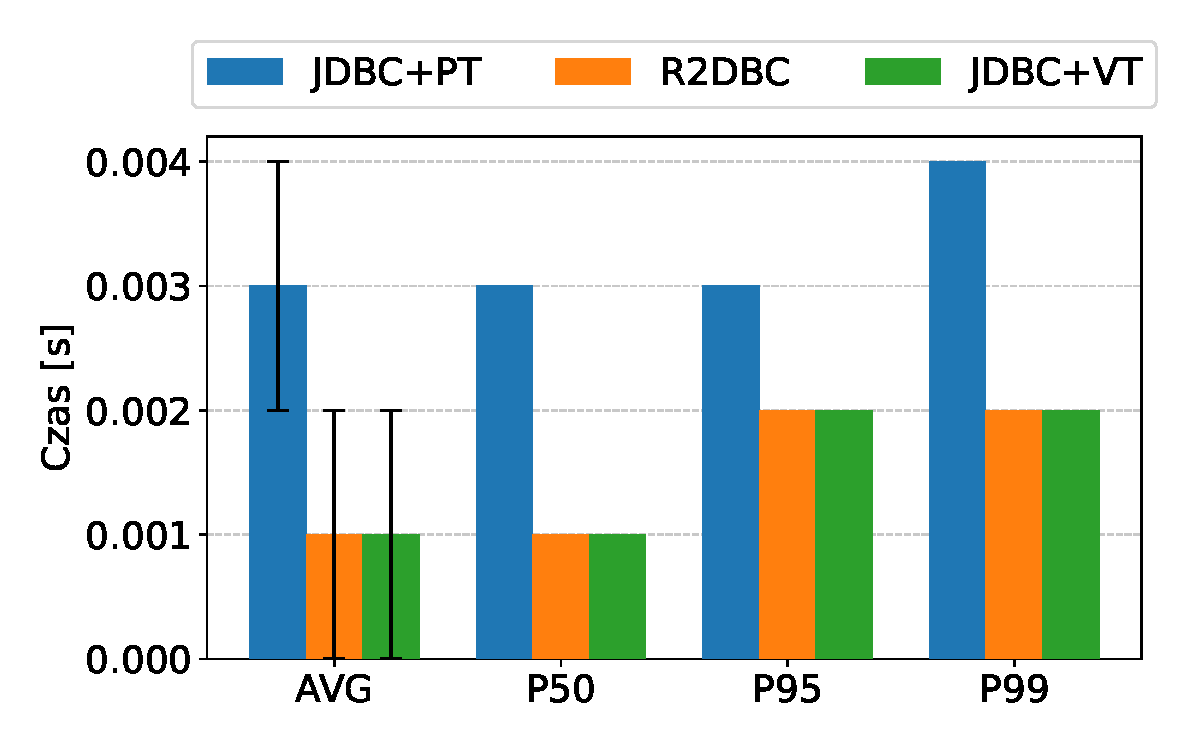
\includegraphics[width=\textwidth]{rozdzialy/rozdzial6/wykresy/A_plot_avg_Q1_16.pdf}
        \caption{poziom współbieżności: 16}
        \label{fig:benchmark-A-sample-Q1-16}
    \end{subfigure}
    \hfill
    \begin{subfigure}[b]{0.49\textwidth}
        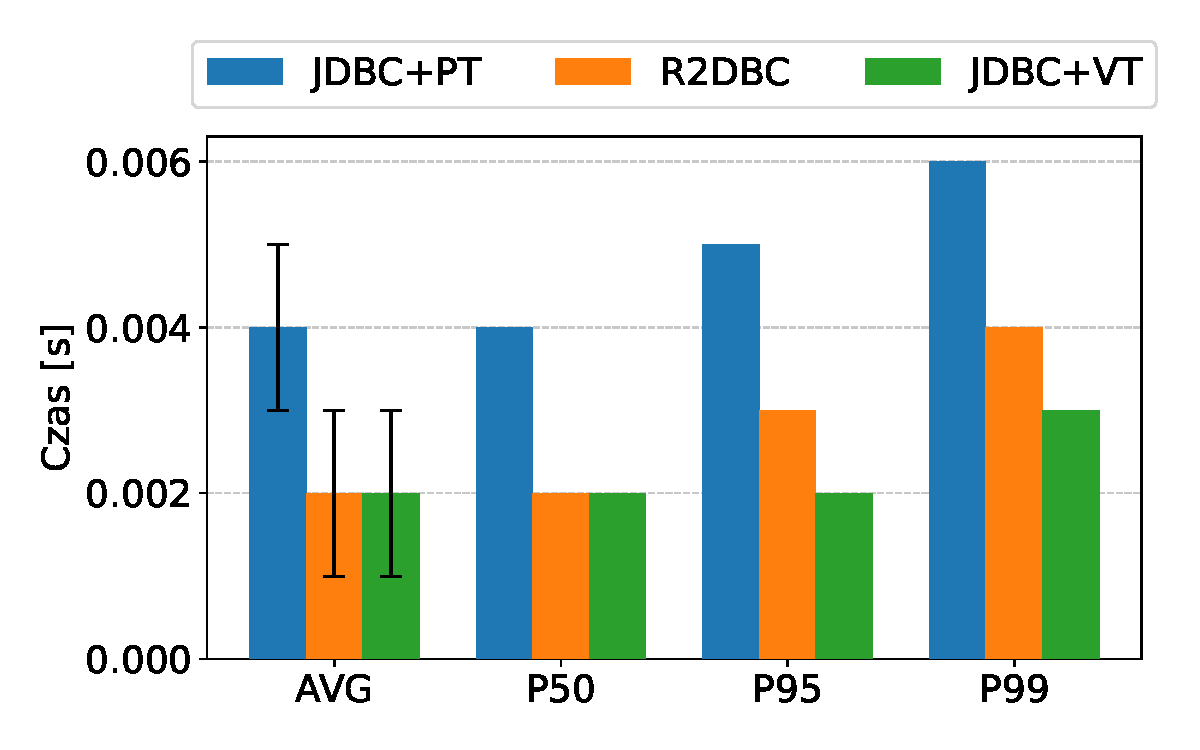
\includegraphics[width=\textwidth]{rozdzialy/rozdzial6/wykresy/A_plot_avg_Q1_32.pdf}
        \caption{poziom współbieżności: 32}
        \label{fig:benchmark-A-sample-Q1-32}
    \end{subfigure}

    \vspace{0.5cm}

    \begin{subfigure}[b]{0.49\textwidth}
        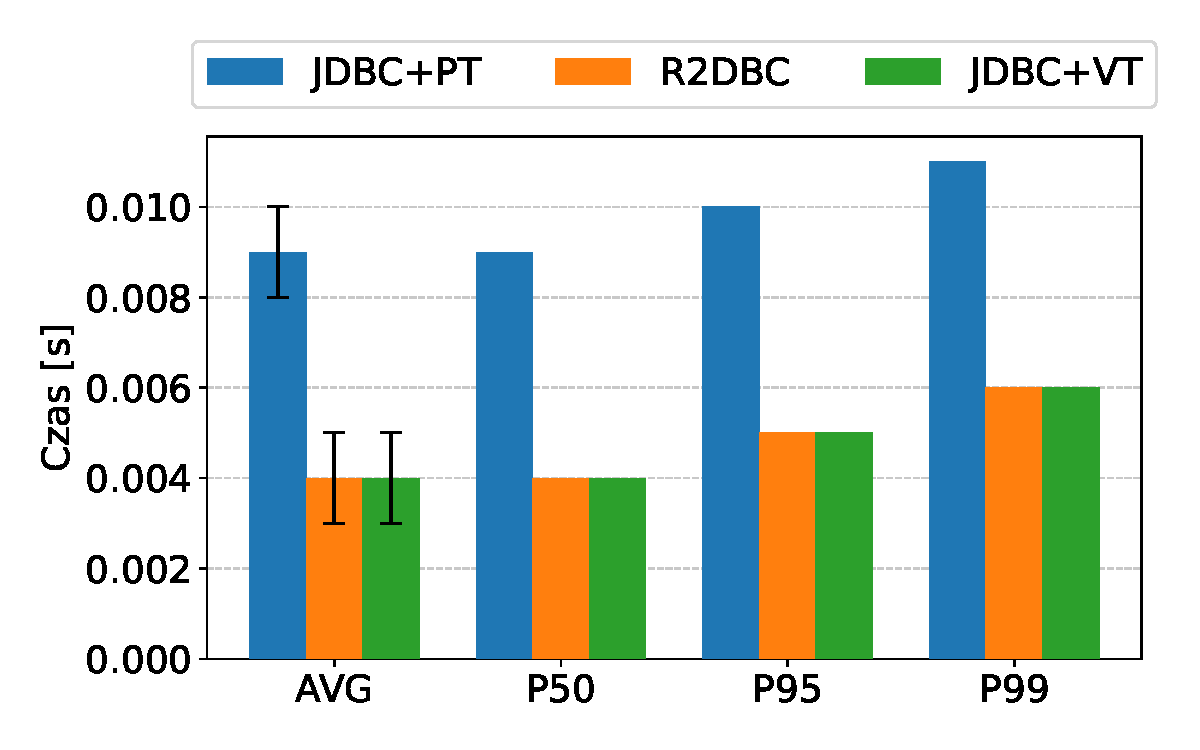
\includegraphics[width=\textwidth]{rozdzialy/rozdzial6/wykresy/A_plot_avg_Q1_64.pdf}
        \caption{poziom współbieżności: 64}
        \label{fig:benchmark-A-sample-Q1-64}
    \end{subfigure}
    \hfill
    \begin{subfigure}[b]{0.49\textwidth}
        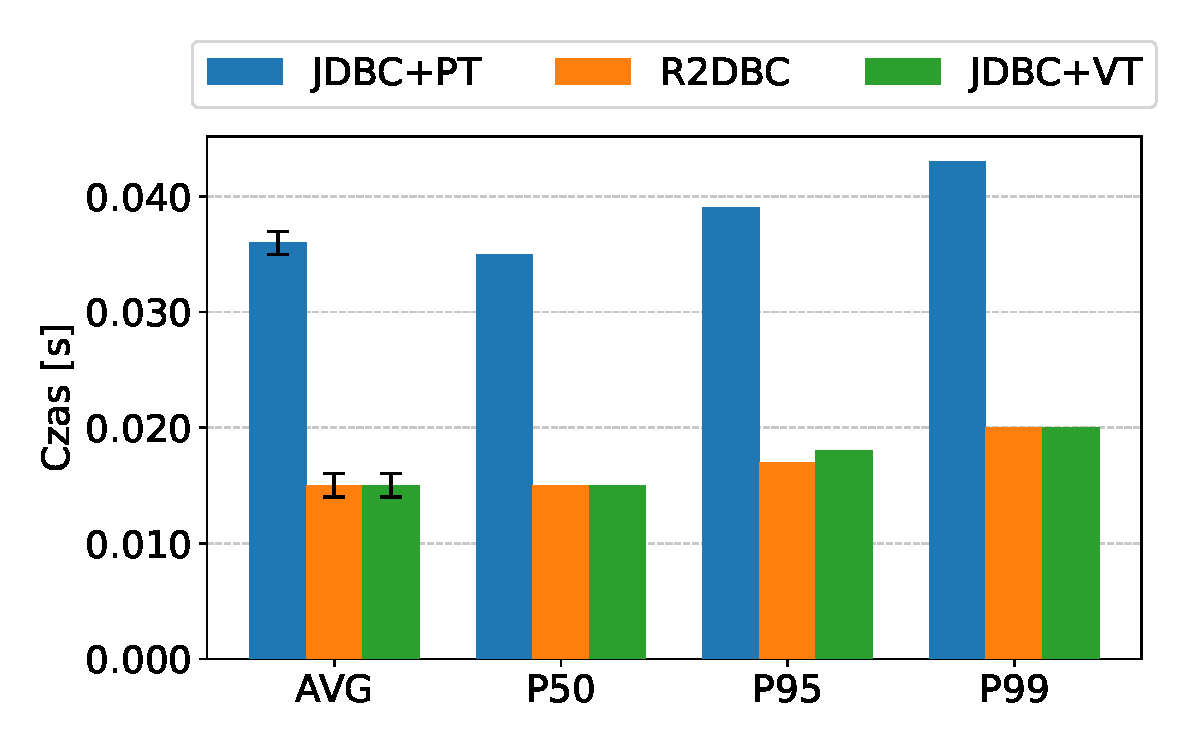
\includegraphics[width=\textwidth]{rozdzialy/rozdzial6/wykresy/A_plot_avg_Q1_256.pdf}
        \caption{poziom współbieżności: 256}
        \label{fig:benchmark-A-sample-Q1-256}
    \end{subfigure}

    \vspace{0.5cm}

    \begin{subfigure}[b]{0.49\textwidth}
        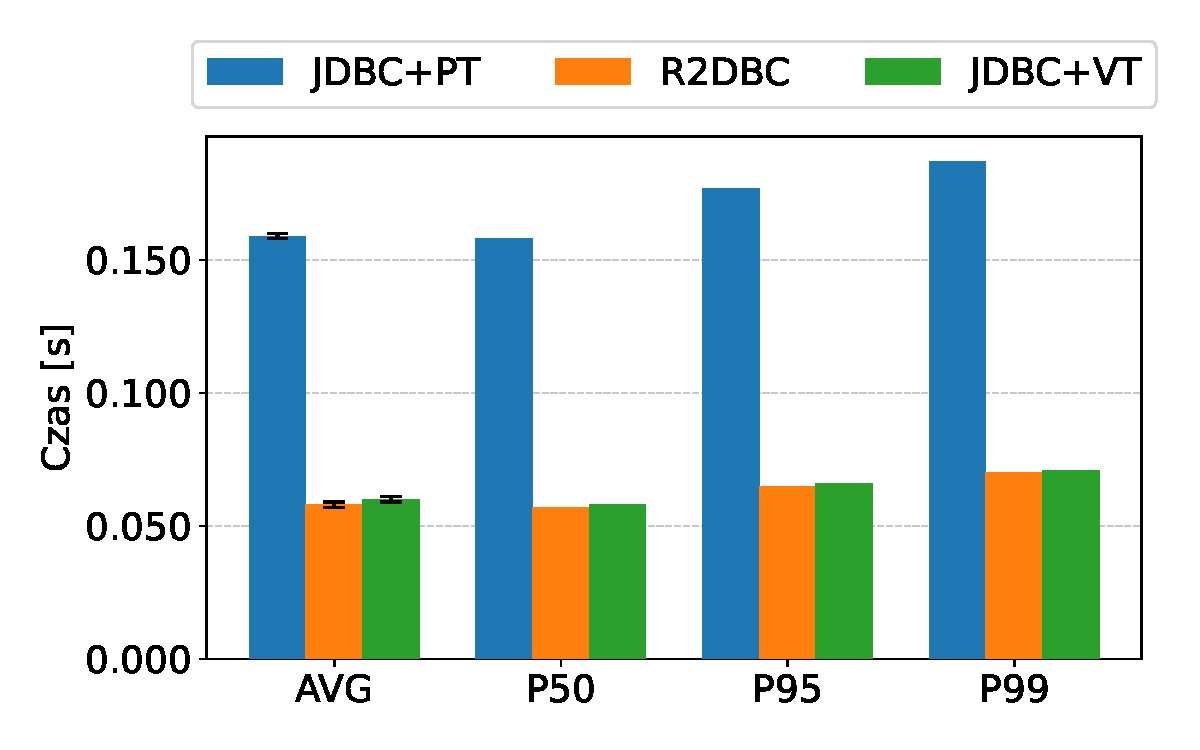
\includegraphics[width=\textwidth]{rozdzialy/rozdzial6/wykresy/A_plot_avg_Q1_1024.pdf}
        \caption{poziom współbieżności: 1024}
        \label{fig:benchmark-A-sample-Q1-1024}
    \end{subfigure}
    \caption{Wykresy kolumnowe średniego czasu i percentyli P50, P95, P99 dla zapytania \texttt{Q1} w~ramach scenariusza $\mathcal{A}$ w~zależności od poziomu współbieżności i~wariantu modelu współbieżności}
    \source{opracowanie własne}
    \label{fig:benchmark-A-sample-Q1}
\end{figure}

\setlength{\tabcolsep}{0.5em} % for the horizontal padding
\renewcommand{\arraystretch}{1.2} % for the vertical padding
\begin{table}[p]
    \centering
    \begin{tabularx}{\linewidth}{|c|c|>{\centering\arraybackslash}X|>{\centering\arraybackslash}X|>{\centering\arraybackslash}X|}
        \hline
        \textbf{Poz. współb.} & \textbf{Metryka} & \textbf{JDBC + PT} & \textbf{R2DBC} & \textbf{JDBC + VT} \\
        \hline
        \multirow{4}{*}{16} & AVG & $0.007 \pm 0.001$ & $0.006 \pm 0.001$ & $0.006 \pm 0.001$ \\ \cline{2-5}
                            & P50 & 0.008 & 0.007 & 0.007 \\ \cline{2-5}
                            & P95 & 0.010 & 0.008 & 0.008 \\ \cline{2-5}
                            & P99 & 0.012 & 0.010 & 0.011 \\
        \hline
        \multirow{4}{*}{32} & AVG & $0.010 \pm 0.001$ & $0.007 \pm 0.001$ & $0.007 \pm 0.001$ \\ \cline{2-5}
                            & P50 & 0.010 & 0.008 & 0.008 \\ \cline{2-5}
                            & P95 & 0.011 & 0.009 & 0.009 \\ \cline{2-5}
                            & P99 & 0.014 & 0.011 & 0.011 \\
        \hline
        \multirow{4}{*}{64} & AVG & $0.019 \pm 0.001$ & $0.013 \pm 0.001$ & $0.014 \pm 0.001$ \\ \cline{2-5}
                            & P50 & 0.019 & 0.014 & 0.014 \\ \cline{2-5}
                            & P95 & 0.021 & 0.016 & 0.016 \\ \cline{2-5}
                            & P99 & 0.025 & 0.020 & 0.022 \\
        \hline
        \multirow{4}{*}{256} & AVG & $0.068 \pm 0.001$ & $0.054 \pm 0.001$ & $0.053 \pm 0.001$ \\ \cline{2-5}
                             & P50 & 0.071 & 0.054 & 0.052 \\ \cline{2-5}
                             & P95 & 0.077 & 0.059 & 0.056 \\ \cline{2-5}
                             & P99 & 0.096 & 0.081 & 0.079 \\
        \hline
        \multirow{4}{*}{1024} & AVG & $0.297 \pm 0.003$ & $0.214 \pm 0.001$ & $0.200 \pm 0.002$ \\ \cline{2-5}
                              & P50 & 0.299 & 0.212 & 0.202 \\ \cline{2-5}
                              & P95 & 0.329 & 0.236 & 0.223 \\ \cline{2-5}
                              & P99 & 0.364 & 0.264 & 0.257 \\
        \hline
    \end{tabularx}
    \caption{Wartości średniego czasu i percentyli P50, P95, P99 dla zapytania \texttt{Q2} w~ramach scenariusza $\mathcal{A}$ w~zależności od poziomu współbieżności i~wariantu modelu współbieżności}
    \source{opracowanie własne}
    \label{table:benchmark-A-sample-Q2}
\end{table}

\begin{figure}[p]
    \centering
    \begin{subfigure}[b]{0.49\textwidth}
        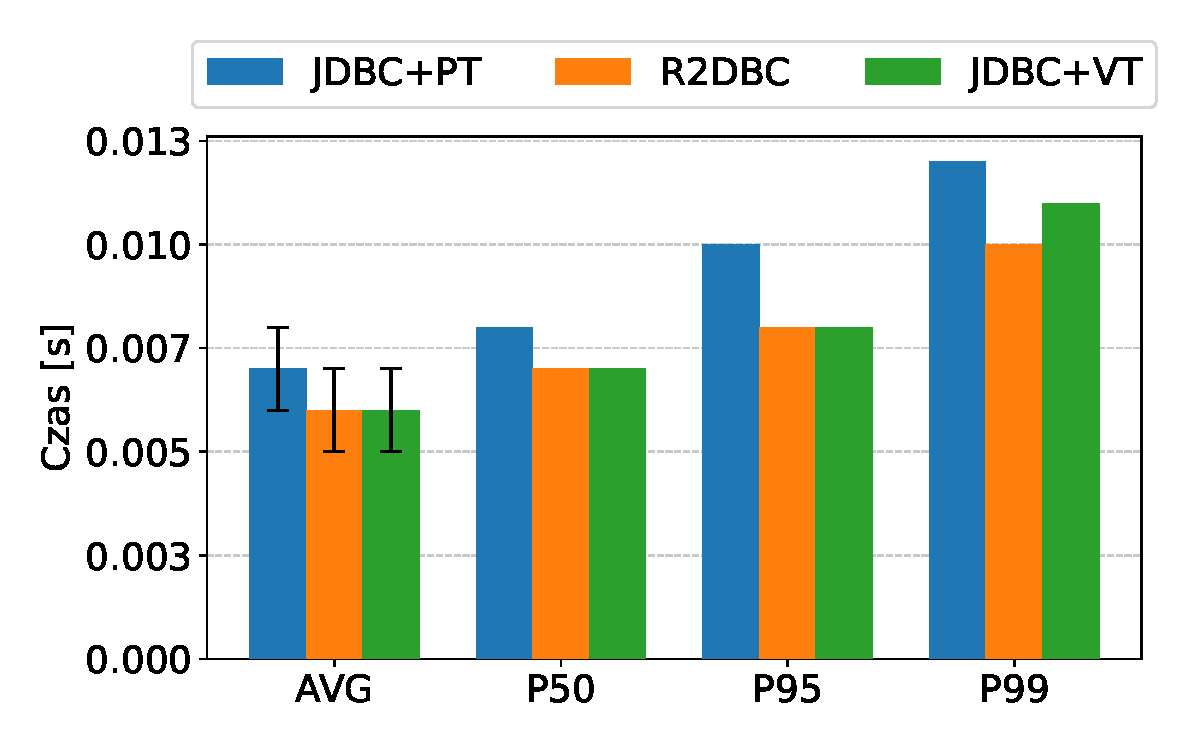
\includegraphics[width=\textwidth]{rozdzialy/rozdzial6/wykresy/A_plot_avg_Q2_16.pdf}
        \caption{poziom współbieżności: 16}
        \label{fig:benchmark-A-sample-Q2-16}
    \end{subfigure}
    \hfill
    \begin{subfigure}[b]{0.49\textwidth}
        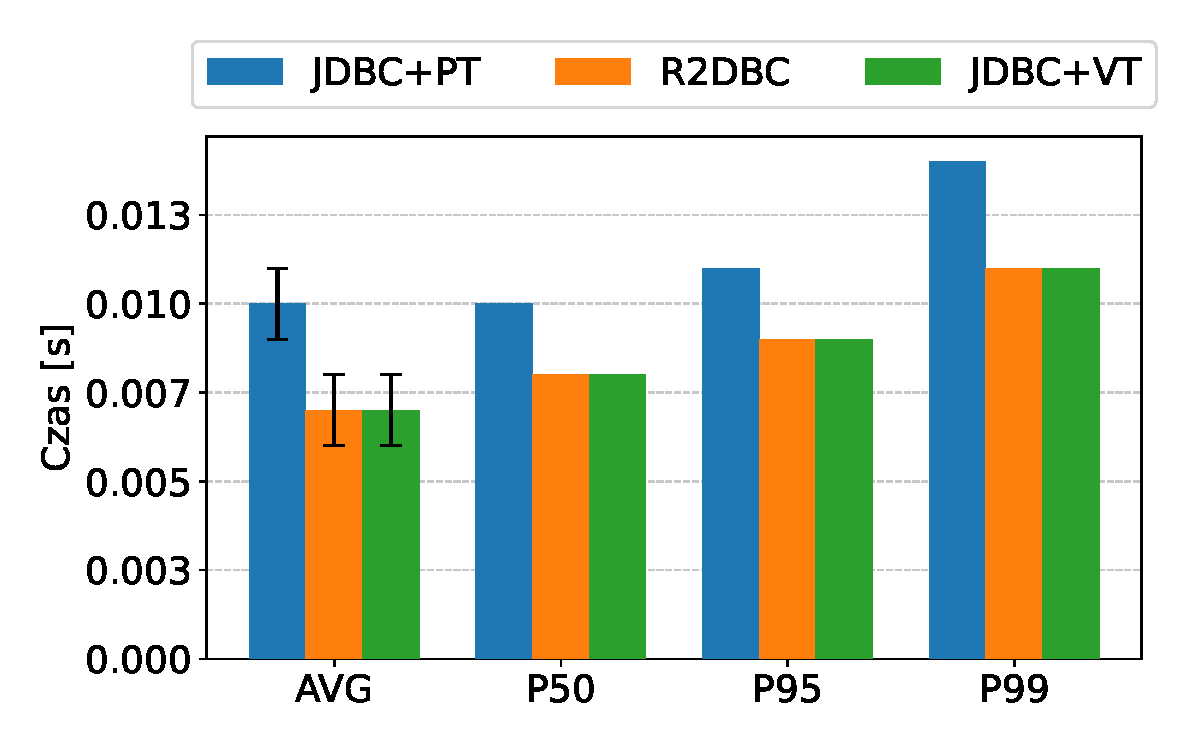
\includegraphics[width=\textwidth]{rozdzialy/rozdzial6/wykresy/A_plot_avg_Q2_32.pdf}
        \caption{poziom współbieżności: 32}
        \label{fig:benchmark-A-sample-Q2-32}
    \end{subfigure}

    \vspace{0.5cm}

    \begin{subfigure}[b]{0.49\textwidth}
        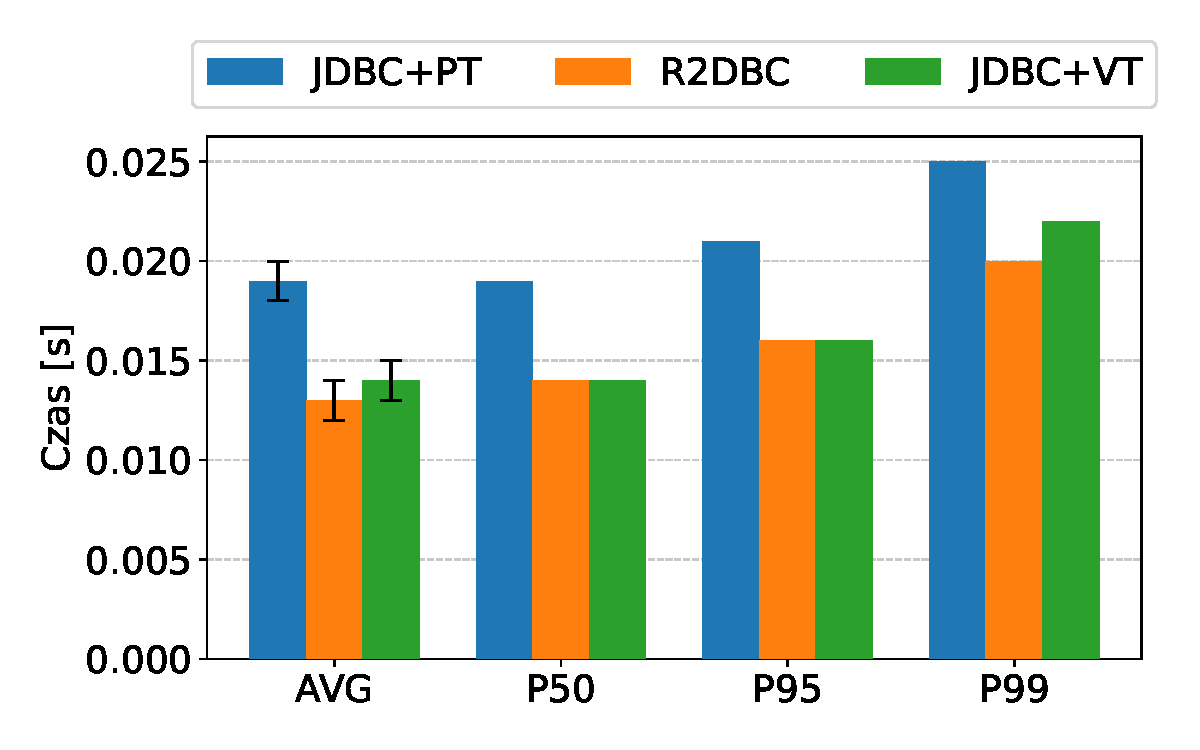
\includegraphics[width=\textwidth]{rozdzialy/rozdzial6/wykresy/A_plot_avg_Q2_64.pdf}
        \caption{poziom współbieżności: 64}
        \label{fig:benchmark-A-sample-Q2-64}
    \end{subfigure}
    \hfill
    \begin{subfigure}[b]{0.49\textwidth}
        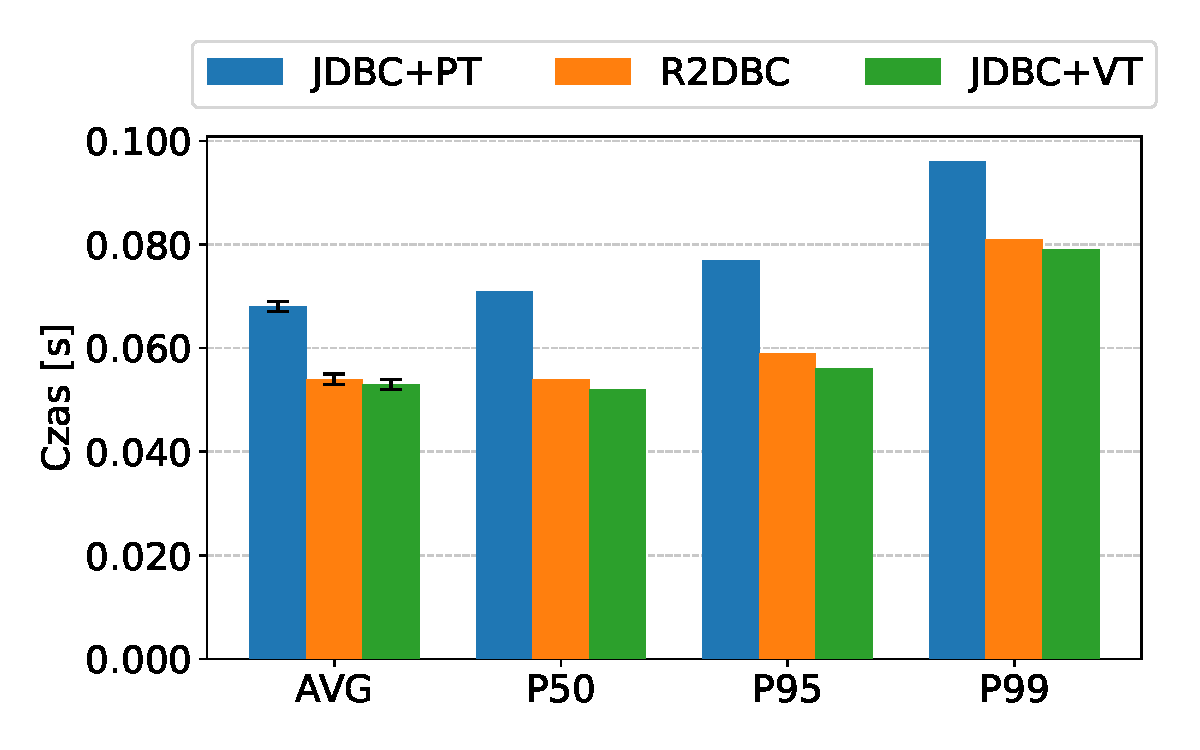
\includegraphics[width=\textwidth]{rozdzialy/rozdzial6/wykresy/A_plot_avg_Q2_256.pdf}
        \caption{poziom współbieżności: 256}
        \label{fig:benchmark-A-sample-Q2-256}
    \end{subfigure}

    \vspace{0.5cm}

    \begin{subfigure}[b]{0.49\textwidth}
        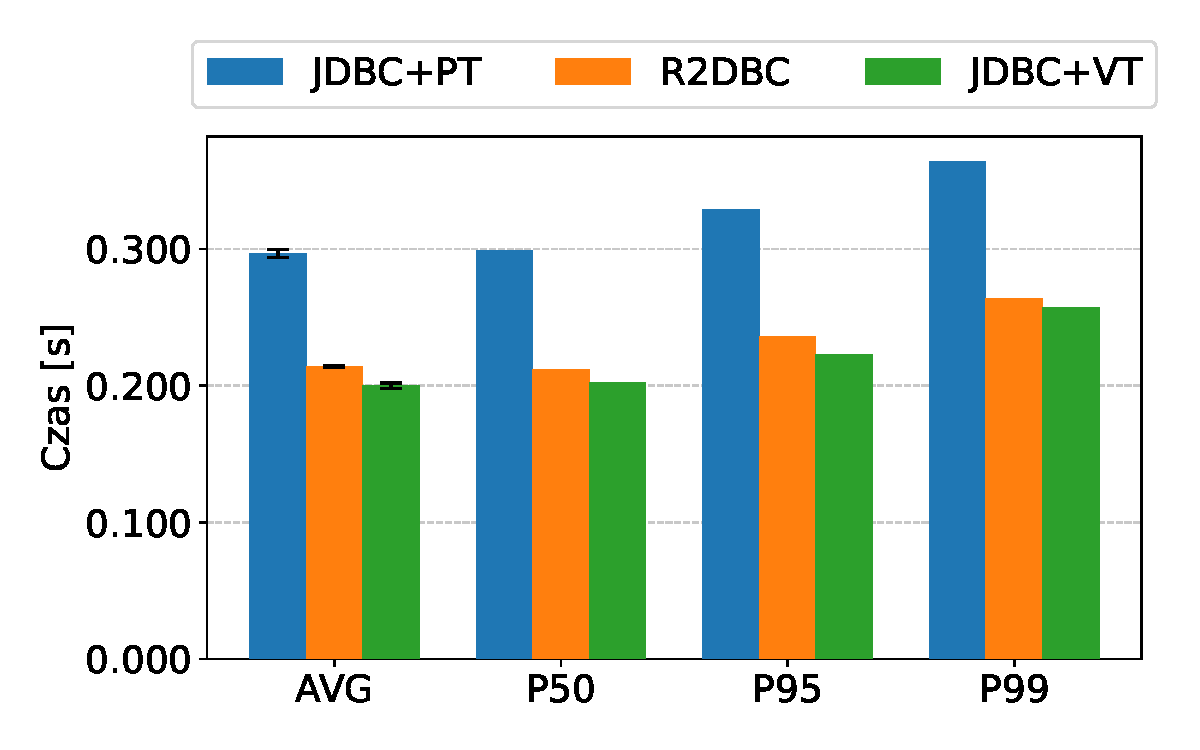
\includegraphics[width=\textwidth]{rozdzialy/rozdzial6/wykresy/A_plot_avg_Q2_1024.pdf}
        \caption{poziom współbieżności: 1024}
        \label{fig:benchmark-A-sample-Q2-1024}
    \end{subfigure}
    \caption{Wykresy kolumnowe średniego czasu i percentyli P50, P95, P99 dla zapytania \texttt{Q2} w~ramach scenariusza $\mathcal{A}$ w~zależności od poziomu współbieżności i~wariantu modelu współbieżności}
    \source{opracowanie własne}
    \label{fig:benchmark-A-sample-Q2}
\end{figure}

\setlength{\tabcolsep}{0.5em} % for the horizontal padding
\renewcommand{\arraystretch}{1.2} % for the vertical padding
\begin{table}[p]
    \centering
    \begin{tabularx}{\linewidth}{|c|c|>{\centering\arraybackslash}X|>{\centering\arraybackslash}X|>{\centering\arraybackslash}X|}
        \hline
        \textbf{Poz. współb.} & \textbf{Metryka} & \textbf{JDBC + PT} & \textbf{R2DBC} & \textbf{JDBC + VT} \\
        \hline
        \multirow{4}{*}{16} & AVG & $0.202 \pm 0.001$ & $0.200 \pm 0.001$ & $0.202 \pm 0.001$ \\ \cline{2-5}
                            & P50 & 0.200 & 0.199 & 0.200 \\ \cline{2-5}
                            & P95 & 0.217 & 0.216 & 0.218 \\ \cline{2-5}
                            & P99 & 0.227 & 0.226 & 0.228 \\
        \hline
        \multirow{4}{*}{32} & AVG & $0.374 \pm 0.001$ & $0.372 \pm 0.001$ & $0.374 \pm 0.001$ \\ \cline{2-5}
                            & P50 & 0.371 & 0.369 & 0.372 \\ \cline{2-5}
                            & P95 & 0.400 & 0.394 & 0.394 \\ \cline{2-5}
                            & P99 & 0.412 & 0.412 & 0.406 \\
        \hline
        \multirow{4}{*}{64} & AVG & $0.757 \pm 0.003$ & $0.751 \pm 0.003$ & $0.760 \pm 0.003$ \\ \cline{2-5}
                            & P50 & 0.753 & 0.748 & 0.755 \\ \cline{2-5}
                            & P95 & 0.784 & 0.778 & 0.793 \\ \cline{2-5}
                            & P99 & 0.820 & 0.820 & 0.830 \\
        \hline
        \multirow{4}{*}{256} & AVG & $3.023 \pm 0.012$ & $2.999 \pm 0.016$ & $3.007 \pm 0.013$ \\ \cline{2-5}
                             & P50 & 3.012 & 2.991 & 3.001 \\ \cline{2-5}
                             & P95 & 3.091 & 3.078 & 3.095 \\ \cline{2-5}
                             & P99 & 3.176 & 3.311 & 3.148 \\
        \hline
        \multirow{4}{*}{1024} & AVG & $5.336 \pm 0.010$ & $11.954 \pm 0.054$ & $5.206 \pm 0.009$ \\ \cline{2-5}
                              & P50 & 5.335 & 11.929 & 5.201 \\ \cline{2-5}
                              & P95 & 5.377 & 12.148 & 5.234 \\ \cline{2-5}
                              & P99 & 5.385 & 12.231 & 5.260 \\
        \hline
    \end{tabularx}
    \caption{Wartości średniego czasu i percentyli P50, P95, P99 dla zapytania \texttt{Q3} w~ramach scenariusza $\mathcal{A}$ w~zależności od poziomu współbieżności i~wariantu modelu współbieżności}
    \source{opracowanie własne}
    \label{table:benchmark-A-sample-Q3}
\end{table}

% \begin{figure}[ht]
%     \centering
%     \includegraphics[width=\textwidth]{rozdzialy/rozdzial6/wykresy/A_plot_avg_Q3.pdf}
%     \caption{Wykres kolumnowy średniego czasu zapytania \texttt{Q3} w zależności od poziomu współbieżności i wariantu modelu współbieżności}
%     \source{opracowanie własne}
%     \label{fig:benchmark-avg-q3}
% \end{figure}

\begin{figure}[p]
    \centering
    \begin{subfigure}[b]{0.49\textwidth}
        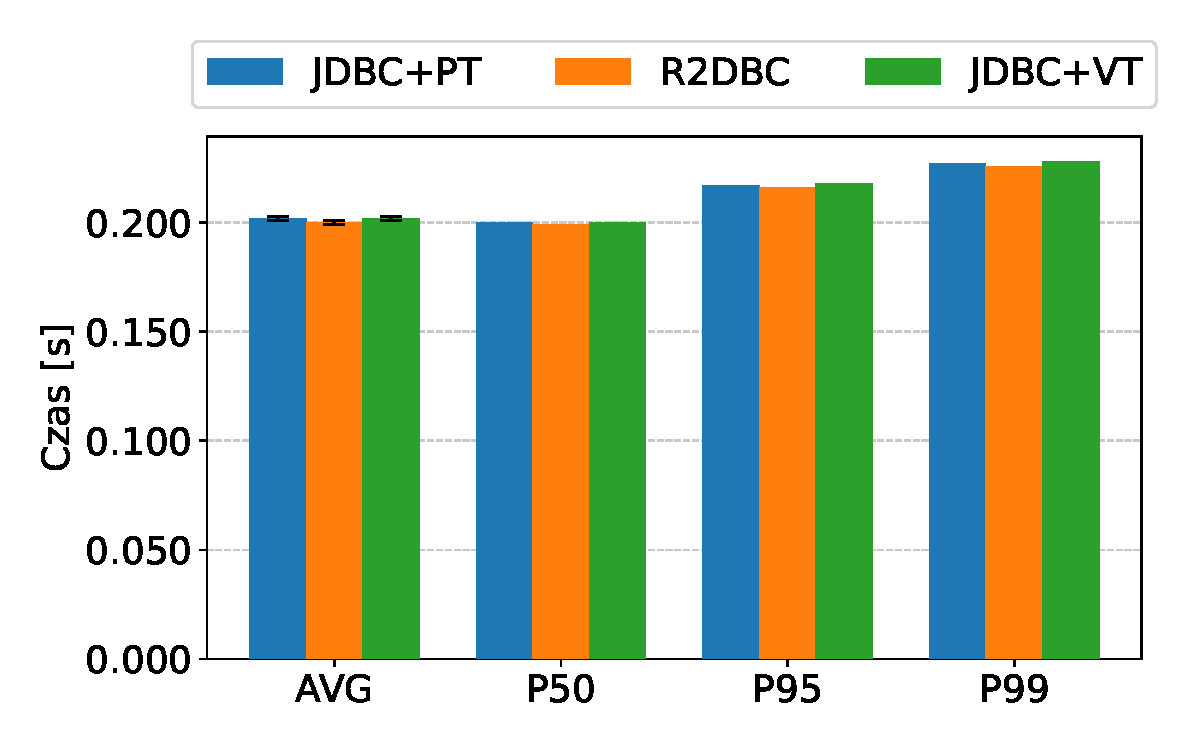
\includegraphics[width=\textwidth]{rozdzialy/rozdzial6/wykresy/A_plot_avg_Q3_16.pdf}
        \caption{poziom współbieżności: 16}
        \label{fig:benchmark-A-sample-Q3-16}
    \end{subfigure}
    \hfill
    \begin{subfigure}[b]{0.49\textwidth}
        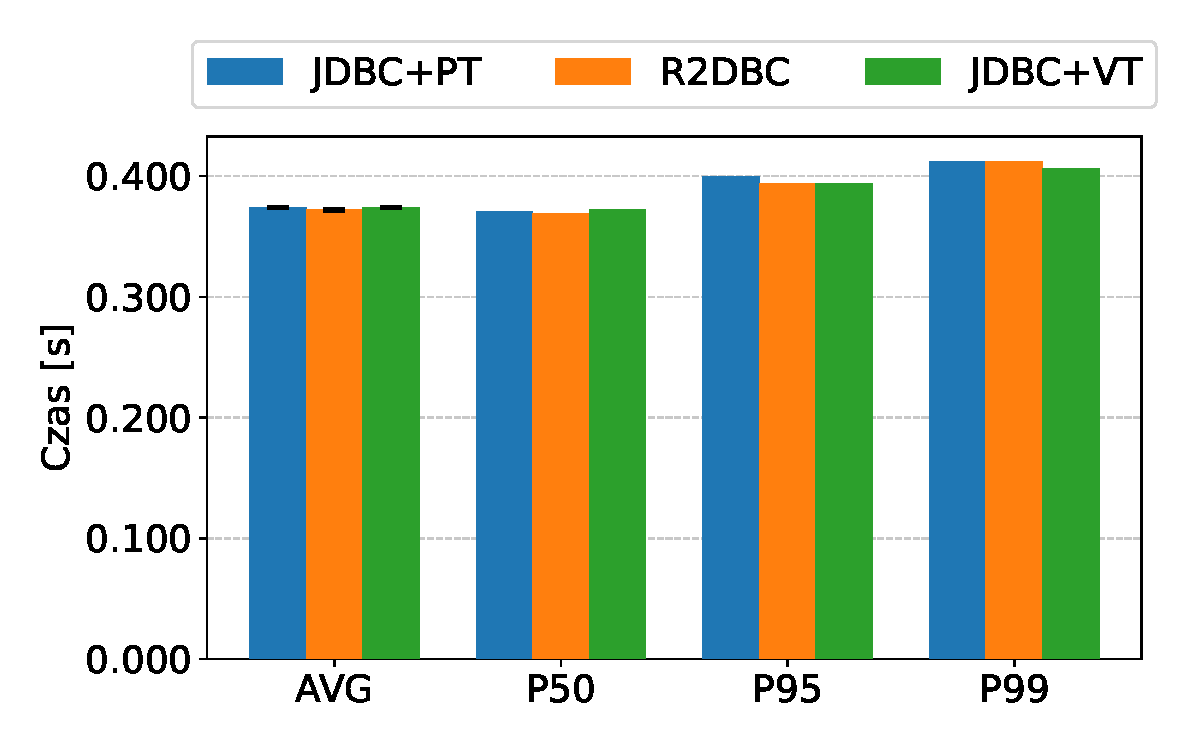
\includegraphics[width=\textwidth]{rozdzialy/rozdzial6/wykresy/A_plot_avg_Q3_32.pdf}
        \caption{poziom współbieżności: 32}
        \label{fig:benchmark-A-sample-Q3-32}
    \end{subfigure}

    \vspace{0.5cm}

    \begin{subfigure}[b]{0.49\textwidth}
        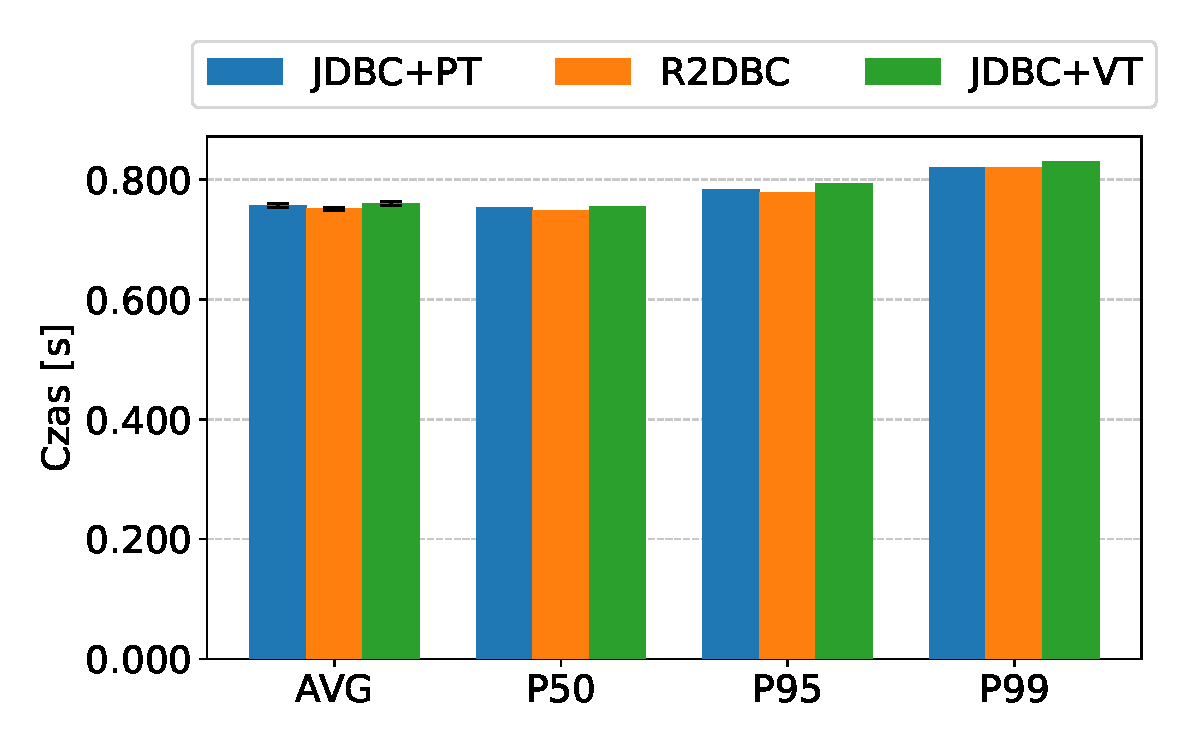
\includegraphics[width=\textwidth]{rozdzialy/rozdzial6/wykresy/A_plot_avg_Q3_64.pdf}
        \caption{poziom współbieżności: 64}
        \label{fig:benchmark-A-sample-Q3-64}
    \end{subfigure}
    \hfill
    \begin{subfigure}[b]{0.49\textwidth}
        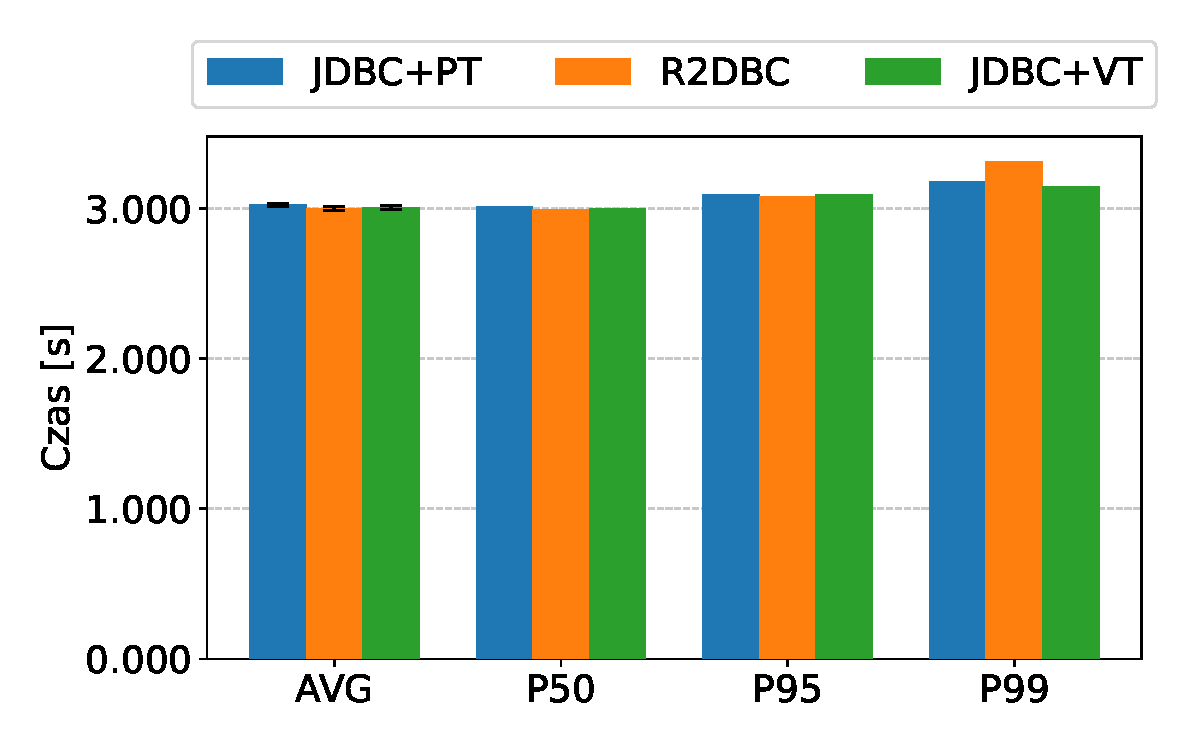
\includegraphics[width=\textwidth]{rozdzialy/rozdzial6/wykresy/A_plot_avg_Q3_256.pdf}
        \caption{poziom współbieżności: 256}
        \label{fig:benchmark-A-sample-Q3-256}
    \end{subfigure}

    \vspace{0.5cm}

    \begin{subfigure}[b]{0.49\textwidth}
        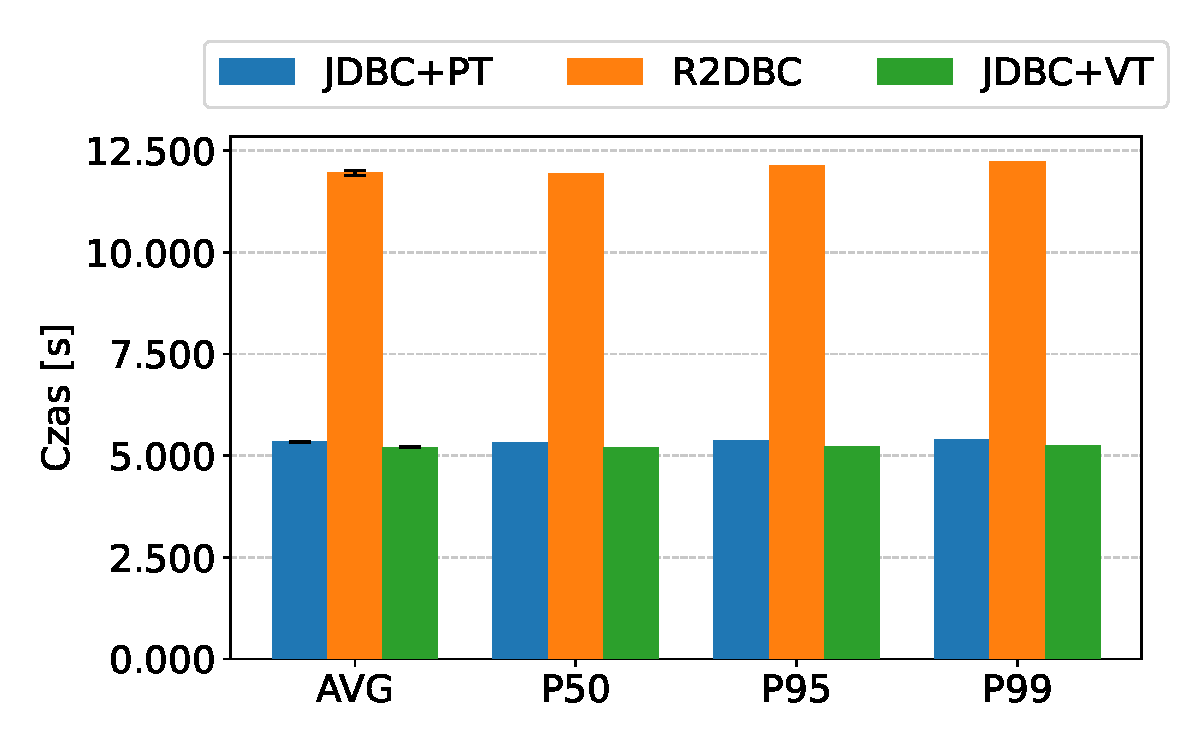
\includegraphics[width=\textwidth]{rozdzialy/rozdzial6/wykresy/A_plot_avg_Q3_1024.pdf}
        \caption{poziom współbieżności: 1024}
        \label{fig:benchmark-A-sample-Q3-1024}
    \end{subfigure}
    \caption{Wykresy kolumnowe średniego czasu i percentyli P50, P95, P99 dla zapytania \texttt{Q3} w~ramach scenariusza $\mathcal{A}$ w~zależności od poziomu współbieżności i~wariantu modelu współbieżności}
    \source{opracowanie własne}
    \label{fig:benchmark-A-sample-Q3}
\end{figure}

\newpage
\subsection{Wyniki pomiarów w ramach scenariusza \ensuremath{\mathcal{B}}}
\label{sec:results-scenario-B}

\subsubsection{Tryb próbkowania czasu (\texttt{SampleTime})}
bla bla bla

\vspace{3cm}
\textit{Wyniki znajdują się na następnej stronie.}

\setlength{\tabcolsep}{0.5em} % for the horizontal padding
\renewcommand{\arraystretch}{1.2} % for the vertical padding
\begin{table}[p]
    \centering
    \begin{tabularx}{\linewidth}{|c|c|>{\centering\arraybackslash}X|>{\centering\arraybackslash}X|>{\centering\arraybackslash}X|}
        \hline
        \textbf{Wariant serwisów} & \textbf{Metryka} & \textbf{Legacy} & \textbf{Reactive} & \textbf{Loom} \\
        \hline
        \multirow{5}{*}{\texttt{THREE\_FAST\_TWO\_SLOW}} & AVG & $0.040 \pm 0.001$ & $0.013 \pm 0.001$ & $0.014 \pm 0.001$ \\ \cline{2-5}
                            & P50   & 0.036 & 0.011 & 0.011 \\ \cline{2-5}
                            & P95   & 0.075 & 0.041 & 0.041 \\ \cline{2-5}
                            & P99   & 0.092 & 0.041 & 0.042 \\ \cline{2-5}
                            & P99.9 & 0.119 & 0.042 & 0.042 \\
        \hline
        \multirow{5}{*}{\texttt{ONE\_FAST\_FOUR\_SLOW}} & AVG & $0.117 \pm 0.003$ & $0.091 \pm 0.001$ & $0.092 \pm 0.001$ \\ \cline{2-5}
                            & P50   & 0.107 & 0.091 & 0.091 \\ \cline{2-5}
                            & P95   & 0.250 & 0.111 & 0.111 \\ \cline{2-5}
                            & P99   & 0.251 & 0.120 & 0.120 \\ \cline{2-5}
                            & P99.9 & 0.252 & 0.216 & 0.217 \\
        \hline
        \multirow{5}{*}{\texttt{FIVE\_SIMILAR}} & AVG & $0.053 \pm 0.001$ & $0.039 \pm 0.001$ & $0.039 \pm 0.001$ \\ \cline{2-5}
                            & P50   & 0.045 & 0.038 & 0.039 \\ \cline{2-5}
                            & P95   & 0.150 & 0.045 & 0.045 \\ \cline{2-5}
                            & P99   & 0.151 & 0.048 & 0.048 \\ \cline{2-5}
                            & P99.9 & 0.153 & 0.051 & 0.052 \\
        \hline
        \multirow{5}{*}{\texttt{OUTLIER\_HEAVY}} & AVG & $0.166 \pm 0.010$ & $0.050 \pm 0.003$ & $0.051 \pm 0.003$ \\ \cline{2-5}
                             & P50   & 0.058 & 0.037 & 0.037 \\ \cline{2-5}
                             & P95   & 0.301 & 0.300 & 0.300 \\ \cline{2-5}
                             & P99   & 0.324 & 0.301 & 0.301 \\ \cline{2-5}
                             & P99.9 & 0.341 & 0.302 & 0.302 \\
        \hline
    \end{tabularx}
    \caption{Wartości średniego czasu i percentyli P50, P95, P99, P99.9 dla scenariusza $\mathcal{B}$ w~zależności od wariantu serwisów i~modelu współbieżności}
    \source{opracowanie własne}
    \label{table:benchmark-B-sample}
\end{table}

% \begin{figure}[ht]
%     \centering
%     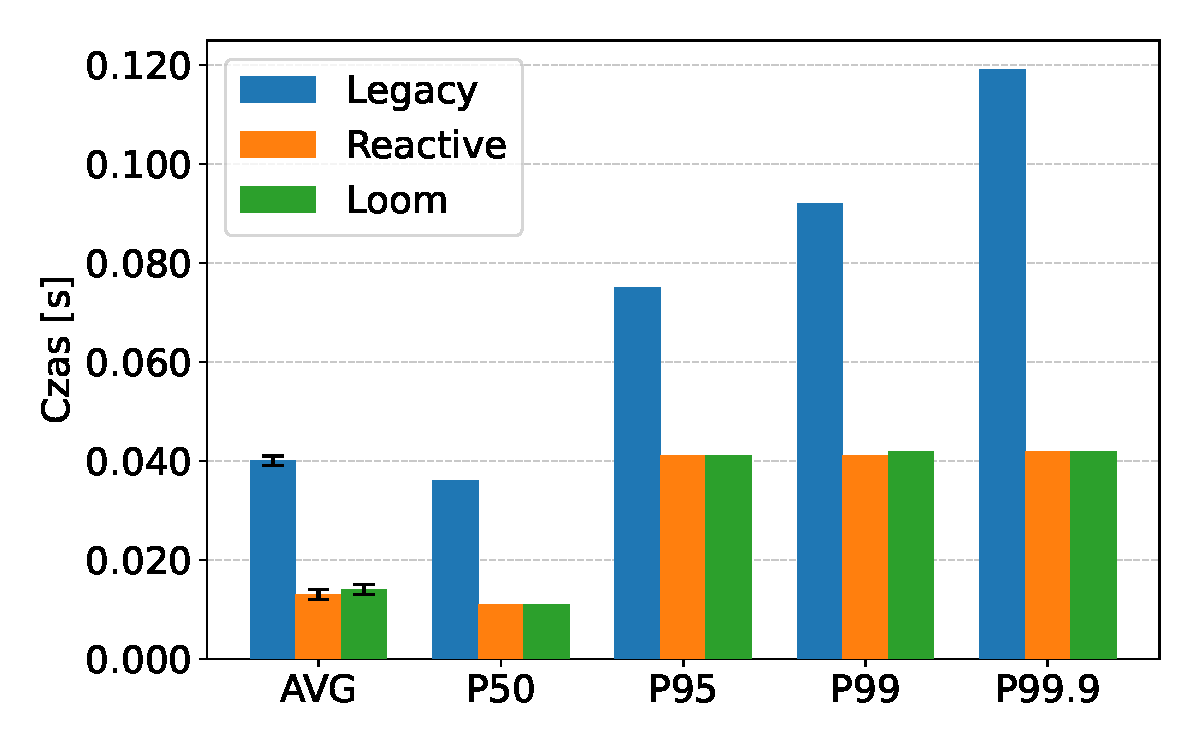
\includegraphics[width=\textwidth]{rozdzialy/rozdzial6/wykresy/B_plot_avg_C1.pdf}
%     \caption{Wykres kolumnowy średniego czasu i latencji P50, P95, P99 i P99.9 dla różnych modeli współbieżności w scenariuszu B dla wariantu \texttt{THREE\_FAST\_TWO\_SLOW}}
%     \source{opracowanie własne}
%     \label{fig:benchmark-B-sample-C1}
% \end{figure}

\begin{figure}[p]
    \centering
    \begin{subfigure}[b]{0.49\textwidth}
        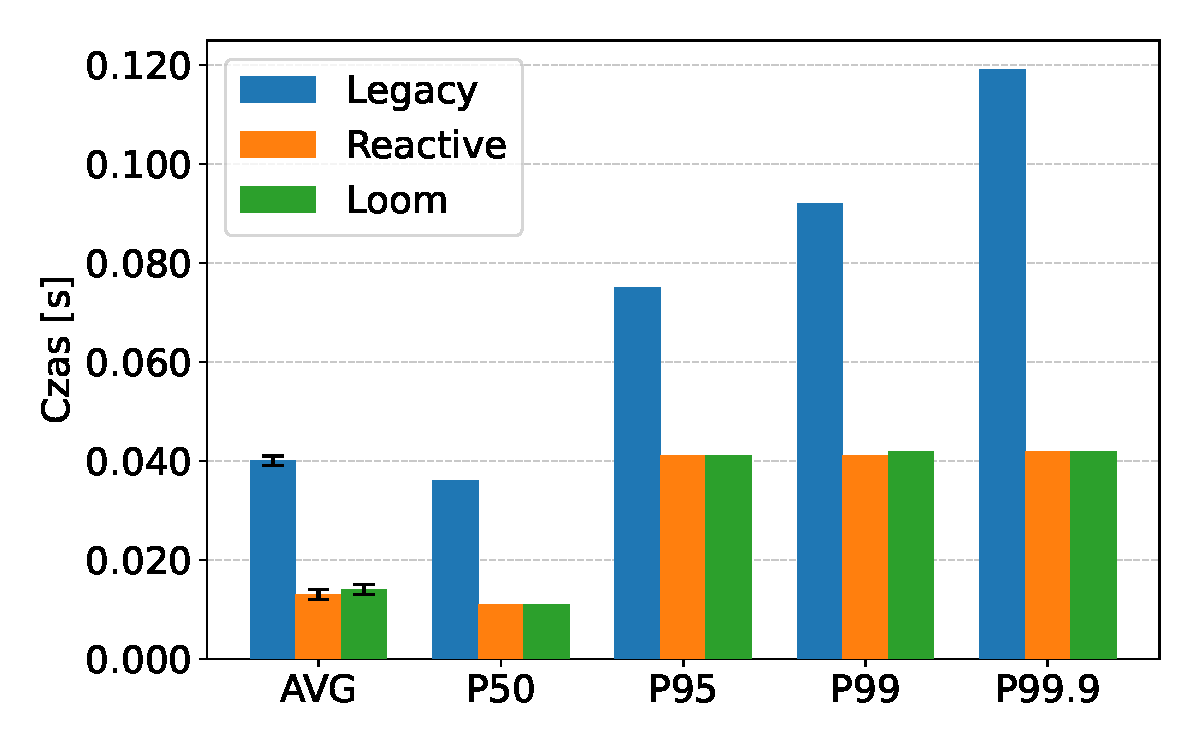
\includegraphics[width=\textwidth]{rozdzialy/rozdzial6/wykresy/B_plot_avg_C1.pdf}
        \caption{wariant \texttt{THREE\_FAST\_TWO\_SLOW}}
        \label{fig:benchmark-B-sample-C1}
    \end{subfigure}
    \hfill
    \begin{subfigure}[b]{0.49\textwidth}
        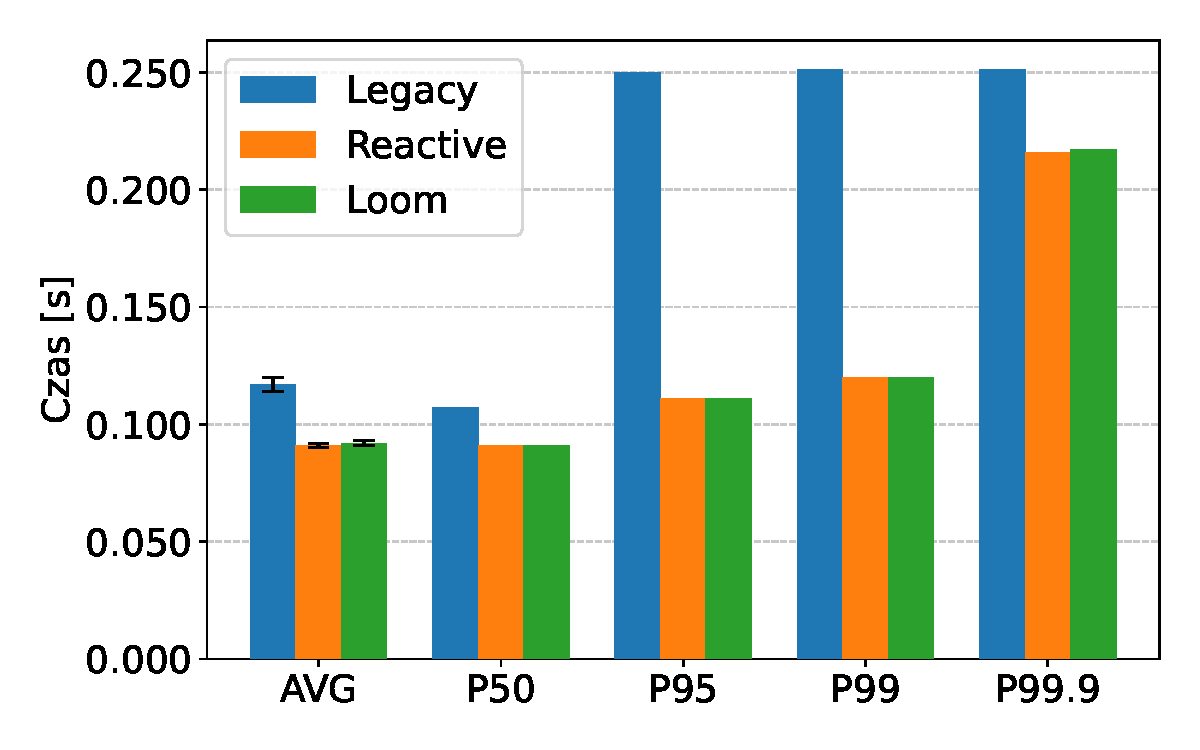
\includegraphics[width=\textwidth]{rozdzialy/rozdzial6/wykresy/B_plot_avg_C2.pdf}
        \caption{wariant \texttt{ONE\_FAST\_FOUR\_SLOW}}
        \label{fig:benchmark-B-sample-C2}
    \end{subfigure}

    \vspace{0.5cm}

    \begin{subfigure}[b]{0.49\textwidth}
        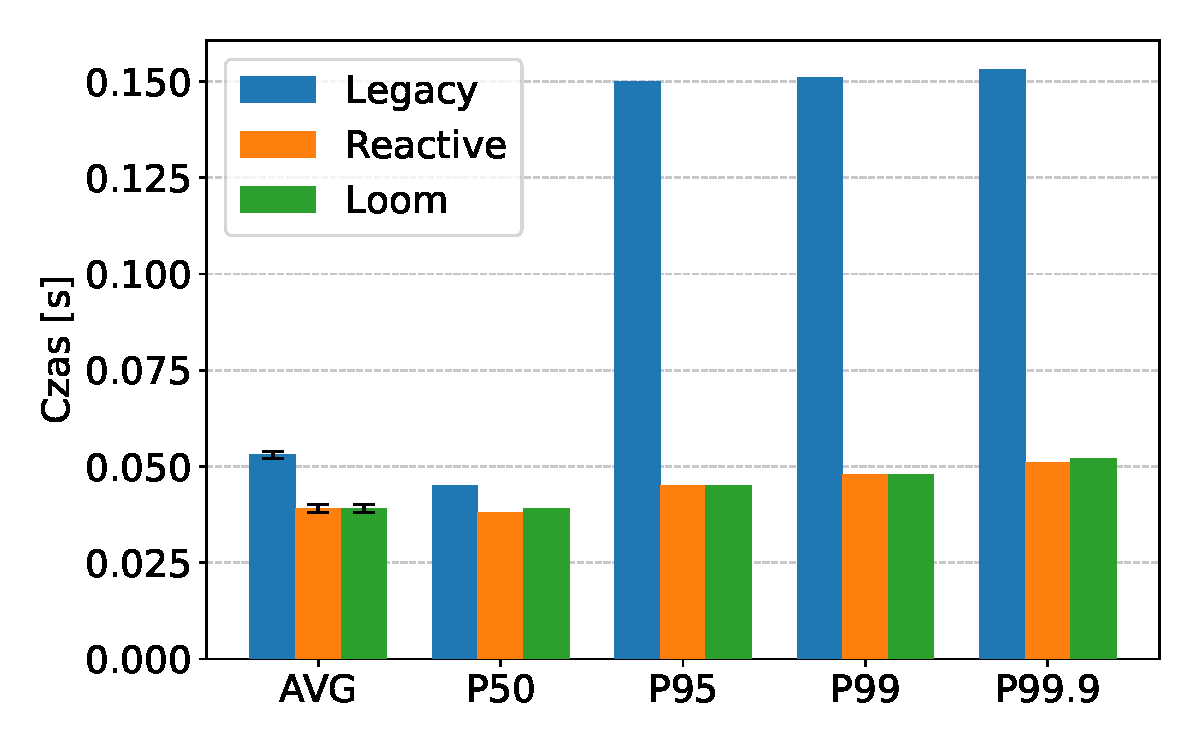
\includegraphics[width=\textwidth]{rozdzialy/rozdzial6/wykresy/B_plot_avg_C3.pdf}
        \caption{wariant \texttt{FIVE\_SIMILAR}}
        \label{fig:benchmark-B-sample-C3}
    \end{subfigure}
    \hfill
    \begin{subfigure}[b]{0.49\textwidth}
        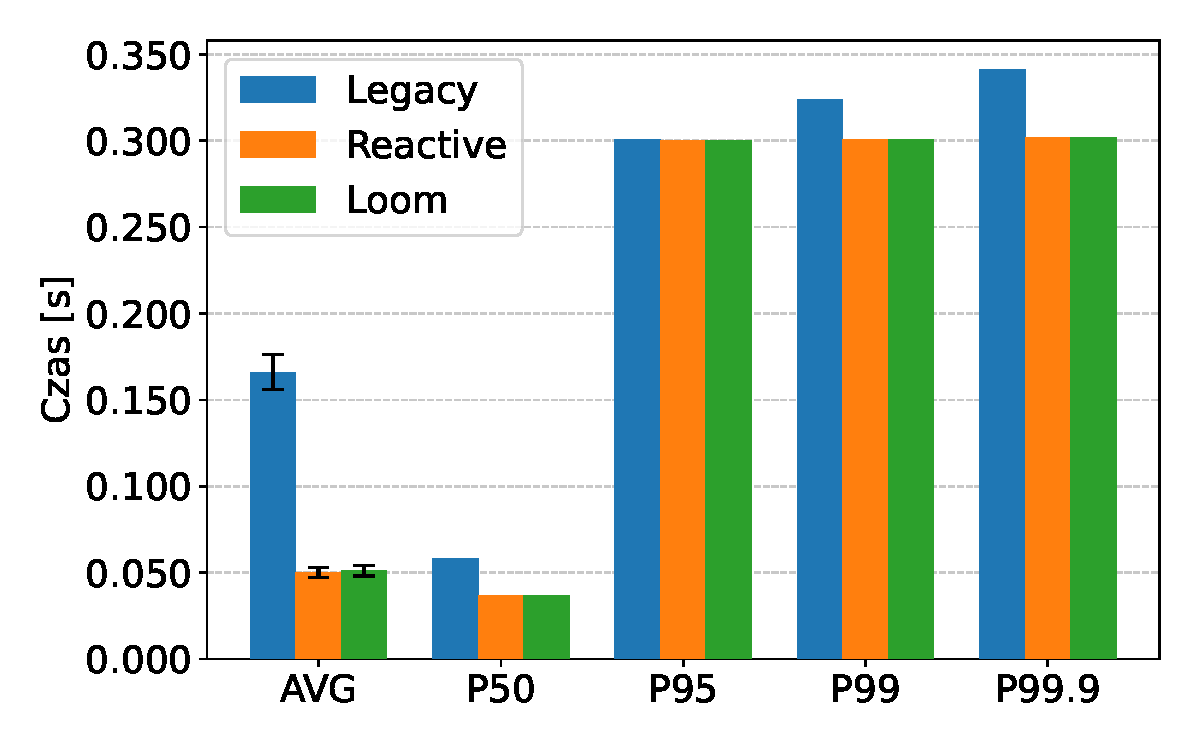
\includegraphics[width=\textwidth]{rozdzialy/rozdzial6/wykresy/B_plot_avg_C4.pdf}
        \caption{wariant \texttt{OUTLIER\_HEAVY}}
        \label{fig:benchmark-B-sample-C4}
    \end{subfigure}
    \caption{Wykresy kolumnowe średniego czasu i percentyli P50, P95, P99, P99.9 dla scenariusza $\mathcal{B}$ w~zależności od wariantu serwisów i~modelu współbieżności}
    \source{opracowanie własne}
    \label{fig:benchmark-B-sample}
\end{figure}

\newpage
\section{Analiza porównawcza i interpretacja wyników}

\subsection{Scenariusz \ensuremath{\mathcal{A}}}

\subsection{Scenariusz \ensuremath{\mathcal{B}}}